\chapter{Storage Management}

\textsc{Perspective}: The implementation of storage management must
accommodate a wide range of allocation requirements.  At the same
time, the implementation must provide generality and some compromise
between ``normal'' programs and those that have unusual
requirements. Although it is clearly sensible to satisfy the needs of
most programs in an efficient manner, there is no way to define what
is typical or to predict how programming style and applications may
change. Indeed, the performance of the implementation may affect both
programming style and applications.

Strings and blocks can be created during program execution at times
that cannot be predicted, in general, from examination of the text of
a program. The sizes of strings and of some types of blocks may vary
and may be arbitrarily large, although practical considerations
dictate some limits. There may be an arbitrary number of strings and
blocks.  The ``lifetimes'' during which they may be used are arbitrary
and are unrelated, in general, to procedure calls and returns.

Different programs vary considerably in the number, type, and sizes of
data objects that are created at run time. Some programs read in
strings, transform them, and write them out without ever creating
other types of objects. Other programs create and manipulate many
lists, sets, and tables but use few strings. Relatively few programs
use co-expressions, but there are applications in which large numbers
of co-expressions are created.

Since a program can construct an arbitrary number of data objects of
arbitrary sizes and lifetimes, some mechanism is needed to allow the
reuse of space for ``dead'' objects that are
no longer accessible to the program. Thus, in addition to a mechanism
for allocating storage for objects at run time, there must be a
storage-reclamation mechanism, which usually is called \textit{garbage
collection}. The methods used for allocation and garbage collection
are interdependent. Simple and fast allocation methods usually require
complex and time-consuming garbage-collection techniques, while more
efficient garbage-collection techniques generally lead to more complex
allocation techniques.

Storage management has influences that are far-reaching. In some
programs, it may account for a major portion of execution time. The
design of data structures, the layout of blocks, and the
representation of strings are all influenced by storage-management
considerations. For example, both a descriptor that points to a block
and the first word of the block contain the same type code. This
information is redundant as far as program execution is concerned,
since blocks are accessed only via descriptors that point to them. The
redundant type information is motivated by storage-management
considerations. During garbage collection, it is necessary to access
blocks directly, rather than through pointers from descriptors, and it
must be possible to determine the type of a block from the block
itself.  Similarly, the size of a block is of no interest in
performing language operations, but the size is needed during garbage
collection. Blocks, therefore, carry some ``overhead'' for storage
management. This overhead consists primarily of extra space,
reflecting the fact that it takes more space to manage storage
dynamically than would be needed if space were allocated
statically. Balancing space overhead against efficiency in allocating
and collecting objects is a complex task.

Such problems have plagued and intrigued implementors since the early
days of LISP. Many ways have been devised to handle dynamic storage
management, and some techniques have been highly refined to meet
specific requirements (Cohen 1981). In the case of Icon, there is
\textit{more }emphasis on storage management for strings than there is
in a language, such as LISP, where lists predominate. Icon's
storage-management system reflects previous experience with
storage-management systems used in XPL (McKeeman, Horning, and Wortman
1970), SNOBOL4 (Hanson 1977), and the earlier Ratfor implementation of
Icon (Hanson 1980). The result is, of course, somewhat idiosyncratic,
but it provides an interesting case study of a real storage-management
system.

\section[11.1 Memory Layout]{11.1 Memory Layout}

During the execution of an Icon program, memory is divided into
several regions. The sizes and locations of these regions are somewhat
dependent on computer architecture and the operating system used, but
typically they have the following form:

\begin{center}
\tablefirsthead{\hline
\centering\arraybslash{\sffamily\bfseries run-time system}\\}
\tablehead{\hline
\centering\arraybslash{\sffamily\bfseries run-time system}\\}
\tabletail{}
\tablelasttail{}
\begin{xtabular}{|m{2.30666in}|}
\hline
\centering\arraybslash{\sffamily\bfseries icode}\\\hline
\centering\arraybslash{\sffamily\bfseries allocated storage}\\\hline
\centering\arraybslash{\sffamily\bfseries free space}\\\hline
\centering\arraybslash{\sffamily\bfseries system stack}\\\hline
\end{xtabular}
\end{center}

This diagram is not drawn to scale; some regions are much larger than others.


\textbf{The Run-Time System}. The run-time system contains the
executable code for the interpreter, built-in operators and functions,
support routines, and so forth. It also contains static storage for
some Icon strings and blocks that appear in C functions.
%% [DonW] Provide another example?
%%For example, the blocks for keyword trapped variables are statically
%%allocated in the data area of the run-time system.
Such blocks never move, but their contents may change. The size of the
run-time system is machine-dependent.

\textbf{The Icode Region}. One of the first things done by the
run-time system is to read in the icode file for the program that is
to be executed. The data in the icode region, which is produced by the
linker, is divided into a number of sections:

\begin{center}
\tablefirsthead{\hline
\centering\arraybslash{\sffamily\bfseries code and blocks}\\}
\tablehead{\hline
\centering\arraybslash{\sffamily\bfseries code and blocks}\\}
\tabletail{}
\tablelasttail{}
\begin{xtabular}{|m{2.2962599in}|}
\hline
\centering\arraybslash{\sffamily\bfseries record information}\\\hline
\centering\arraybslash{\sffamily\bfseries global identifier values}\\\hline
\centering\arraybslash{\sffamily\bfseries global identifier names}\\\hline
\centering\arraybslash{\sffamily\bfseries static identifier values}\\\hline
\centering\arraybslash{\sffamily\bfseries strings}\\\hline
\end{xtabular}
\end{center}

The first section contains virtual machine code, blocks for cset and
real literals, and procedure blocks, on a per-procedure basis. Thus,
the section of the icode region that contains code and blocks consists
of segments of the following form for each procedure:

\begin{center}
\tablefirsthead{\hline
\centering\arraybslash{\sffamily\bfseries blocks for real literals}\\}
\tablehead{\hline
\centering\arraybslash{\sffamily\bfseries blocks for real literals}\\}
\tabletail{}
\tablelasttail{}
\begin{xtabular}{|m{2.2858598in}|}
\hline
\centering\arraybslash{\sffamily\bfseries blocks for cset literals}\\\hline
\centering\arraybslash{\sffamily\bfseries procedure blocks}\\\hline
\centering\arraybslash{\sffamily\bfseries virtual machine instructions}\\\hline
\end{xtabular}
\end{center}

Record information for the entire program is in the second section of
the icode region. Next, there is an array of descriptors for the
values of the global identifiers in the program, followed by an array
that contains qualifiers for the names of the global
identifiers. These two arrays are parallel. The \textit{ith}
descriptor in the first array contains the value of the ith global
identifier, and the ith descriptor in the second array contains a
qualifier for its name.

Following the two arrays related to global identifiers is an array for
the values of static identifiers. As mentioned in Sec. 2.1.10, static
identifiers have global scope with respect to procedure invocation,
but a static identifier is accessible only to the procedure in which
it is declared.

Unlike cset and real blocks, which are compiled on a per-procedure
basis, all strings in a program are pooled and are in a single section
of the icode region that follows the array of static identifiers. A
literal string that occurs more than once in a program occurs only
once in the string section of the icode region.

Data in the icode region is never moved, although some components of
it may change at run time. The size of the icode region depends
primarily on the size of the corresponding source program. As a rule
of thumb, an icode region is approximately twice as large as the
corresponding Icon source-language file. An icode file for a short
program might be 1,000 bytes, while one for a large program (by Icon
standards) might be 20,000 bytes.

\textbf{Allocated Storage.} The space for data objects that are
constructed at run time is provided in allocated storage regions. This
portion of memory is divided into three parts:

\begin{center}
\tablefirsthead{\hline
\centering\arraybslash{\sffamily\bfseries static region}\\}
\tablehead{\hline
\centering\arraybslash{\sffamily\bfseries static region}\\}
\tabletail{}
\tablelasttail{}
\begin{xtabular}{|m{2.2858598in}|}
\hline
\centering\arraybslash{\sffamily\bfseries string region}\\\hline
\centering\arraybslash{\sffamily\bfseries block region}\\\hline
\end{xtabular}
\end{center}

The static region contains co-expression blocks. The remainder of the
allocated storage region is divided into strings and blocks as
shown. The string region contains only characters. The block region,
on the other hand, contains pointers. This leads to a number of
differences in allocation and garbage-collection techniques in
different regions.

Data in the static region is never moved, but strings and blocks may
be. Both the string and block regions may be moved if it is necessary
to increase the size of the static region. Similarly, the block region
may be moved in order to enlarge the string region.

The initial sizes of the allocated storage regions vary considerably
from computer to computer, depending on the size of the user address
space. On a computer with a small address space, such as the PDP-ll,
Icon was implemented with region sizes as small as:

\begin{tabular}{l@{\hspace{1cm}}l@{\hspace{1cm}}l}
static region: & 4,096 bytes & (2,048 words)\\
string region: & 10,240 bytes & (5,120 words)\\
block region: & 10,240 bytes & (5,120 words)\\
\hline
total: & 24,576 bytes & (12,288 words)\\
\end{tabular}
\bigskip

On modern machines, initial sizes of 500,000 bytes or 2,000,000 bytes
per region are common. Unicon allocates 1\% of physical memory for
each of the string and block region. The user may establish different
initial sizes prior to program execution by using environment
variables STRSIZE and BLKSIZE. As indicated previously, the sizes of
these regions are increased at run time if necessary, but there is no
provision for decreasing the size of a region once it has grown to a
given size.

\textbf{Free Space and the System Stack}. On computers with system
stacks that grow downward, such as the VAX, the system stack grows
toward the allocated storage region. Between the two regions is a
region of free space into which the allocated storage region may grow
upward. Excessive recursion in C may cause collision of the system
stack and the allocated storage region. This is an unrecoverable
condition, and the result is termination of program execution.
Similarly, more space may be needed for allocated storage than is
available. This also results in termination of program execution. In
practice, the actual situation depends to a large extent on the size
of the user address space, which is the total amount of memory that is
available for all the regions shown previously. On a computer with a
small user address space, such as the PDP-11, the amount of memory
available for allocated storage is a limiting factor for some
programs. Furthermore, collision of the allocated storage region and
the system stack is a serious problem. On a computer that supports a
large virtual memory, the size of the system stack is deliberately
limited, since the the total amount of memory available is so large
that runaway recursion would consume enormous resources before a
collision occurred between the system stack and the allocated storage
region.

\section[11.2 Allocation]{11.2 Allocation}

Storage allocation in Icon is designed to be fast and simple. Garbage
collection is somewhat more complicated as a result. Part of the
rationale for this approach is that most Icon programs do a
considerable amount of allocation, but many programs never do a
garbage collection. Hence, programs that do not garbage collect are
not penalized by a strategy that makes garbage collection more
efficient at the expense of making allocation less efficient. The
other rationale for this approach is that the storage requirements of
Icon do not readily lend themselves to more complex allocation
strategies.

\subsection[11.2.1 The Static Region]{11.2.1 The Static Region}

Data allocated in the static region is never moved, although it may be
freed for reuse. Co-expression blocks are allocated in the static
region, since their C stacks contain internal pointers that depend on
both the computer and the C compiler and hence are difficult to
relocate to another place in memory. Furthermore, since co-expression
blocks are all the same size, it is economical and simple to free and
reuse their space.

The C library routines \texttt{malloc()} and \texttt{free()} are used
to allocate and free co-expression blocks in the static region. These
routines maintain a list of blocks of free space. The routine
\texttt{malloc()} finds a block of the requested size, dividing a
larger block if necessary, and revises the free list accordingly. The
routine \texttt{free()} returns the freed space to the free list,
coalescing it with adjacent free blocks if possible. See Kernighan and
Ritchie 1978 for a discussion of free-list allocation.

Icon contains its own version of these routines to assure that space
is allocated in its own static region and to allow its overall memory
region to be expanded without conflict with other users of
\texttt{malloc()}. Thus, if a user extension to Icon or the operating
system calls \texttt{malloc()}, Icon's own routine handles the
request. This means that the static region may contain space allocated
for data other than co-expression blocks, although this normally is
not the case.

\subsection[11.2.2 Blocks]{11.2.2 Blocks}

For other kinds of blocks, Icon takes advantage of the fact that its
own data can be relocated if necessary and uses a very simple
allocation technique. The allocated region for blocks is divided into
two parts:

\begin{center}
\begin{picture}(400,105)
\put(150,-8){\line(0,1){120}}
\put(250,-8){\line(0,1){120}}
\put(150,2){\line(1,0){100}}
\put(150,102){\line(1,0){100}}
\put(160,25){\shortstack{allocated blocks \\ \\ \\ \\ \\ \\ \\ \\ \\ \\ \\ \\ \\ \\ free block space}}
\put(150,60){\dashbox{2.5}(100,0){}}
\put(75,57.5){\texttt{blkfree}}
\put(80,0){\texttt{blkend}}
\put(75,99){\texttt{blkbase}}
\thicklines
\put(120,60){\vector(1,0){28}}
\put(120,2){\vector(1,0){28}}
\put(120,102){\vector(1,0){28}}
\end{picture}
\end{center}

When there is a request for a block of \textit{n} bytes, the free
pointer, \texttt{blkfree}, is incremented by \textit{n} and the
previous value of the free pointer is returned as the location of the
newly allocated block. This process is fast and free of the
complexities of the free-list approach.


Note that this technique really amounts to a free list with only one
block. The problem of reclaiming fragmented space on the free list is
exchanged for the process of reclaiming unused blocks and rearranging
the block region so that all the free space is in one contiguous
portion of the block region. This is done during garbage collection.

\subsection[11.2.3 Strings]{11.2.3 Strings}

There is even less justification for a free-list approach for
allocating strings. A newly created string may be one character long
or it may be thousands of characters long. Furthermore, while there is
space in blocks that can be used to link together free storage, there
is no such space in strings, and a free list would involve additional
storage.

Instead, the string region is allocated in the same way that the block
region is allocated:

\begin{center}
%--%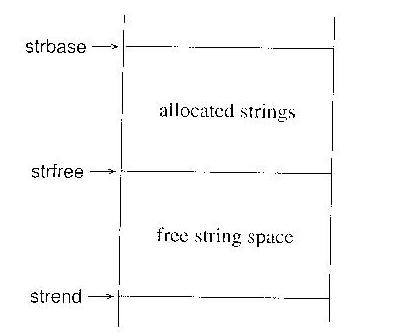
\includegraphics[width=2.1799in,height=1.7492in]{ib-img/ib-img089.jpg}
\begin{picture}(400,105)
\put(150,-8){\line(0,1){120}}
\put(250,-8){\line(0,1){120}}
\put(150,2){\line(1,0){100}}
\put(150,102){\line(1,0){100}}
\put(160,25){\shortstack{allocated strings \\ \\ \\ \\ \\ \\ \\ \\ \\ \\ \\ \\ \\ \\ free string space}}
\put(150,60){\dashbox{2.5}(100,0){}}
\put(75,57.5){\texttt{strfree}}
\put(80,0){\texttt{strend}}
\put(75,99){\texttt{strbase}}
\thicklines
\put(120,60){\vector(1,0){28}}
\put(120,2){\vector(1,0){28}}
\put(120,102){\vector(1,0){28}}
\end{picture}
\end{center}

As with the block region, a garbage collection is performed if there
is not enough space in the string region to satisfy an allocation
request.


\section[11.3 Garbage Collection]{11.3 Garbage Collection}

Allocation is simple, but garbage collection is not. The primary
purpose of garbage collection is to reclaim the space occupied by
``dead'' objects that are not needed for subsequent program execution,
so that this space can be reallocated. This means different things in
different regions. In the static region, it means freeing dead
co-expression blocks. In the string and block regions, it involves
moving the space for dead objects from the allocated portion of the
region to the free portion. This is considerably more complicated than
adding a pointer to a free list. Since all free space must be in a
single block in these regions, ``live'' objects must be moved to fill
in the holes left by dead ones. This is done by compacting the
allocated portion of these regions, relocating live objects toward the
beginning of these regions and squeezing out dead objects. In turn,
pointers to live objects have to be adjusted to correspond to their
new locations. There are two phases in garbage collection:

\liststyleLxii
\begin{itemize}
\item 
\ \ Location of live objects and all the pointers to them.
\item 
\ \ Compaction of live objects and adjustment of the pointers to them.
\end{itemize}

``Garbage collection'' is somewhat of a misnomer, since the process is
oriented toward saving ``non-garbage'' objects; garbage disappears as
a byproduct of this operation.

\subsection[11.3.1 The Basis]{11.3.1 The Basis}

The challenging problem for garbage collection is the location of
objects that have to be saved, as well as all pointers to them. An
object is dead, by definition, if it cannot be accessed by any future
source-language computation.  Conversely, by definition, an object is
live if it can be accessed. Consequently, the important issue is the
possibility of computational access. For example, it is always
possible to access the value of \texttt{\&subject}, and this value
must be preserved by garbage collection. On the other hand, in

%-% {\ttfamily\mdseries
%-% \ \ \ a := [1,2,3]}
%-% 
%-% {\ttfamily\mdseries
%-% \ \ \ a := list(10)}
\goodbreak
\iconcode{
\>a := [1,2,3]\\
\>a := list(10)
}

\noindent after the execution of the second assignment, the first list
assigned to a is inaccessible and can be collected.

It is essential to save any object that may be accessed, but there is
no way, in general, to know if a specific object \textit{will} be
accessed. For example, a computational path may depend on factors that
are external to the program, such as the value of data that is read
from a file. It does comparatively little harm to save an object that
might be accessed but, in fact, never is. Some storage is wasted, but
it is likely to be reclaimed during a subsequent collection. It is a
serious error, on the other hand, to discard an object that
subsequently \textit{is} accessed. In the first place, the former
value of such an object usually is overwritten and hence is
``garbage'' if it is subsequently accessed. Furthermore, accessing
such an object may overwrite another accessible object that now
occupies the space for the former one. The effects may range from
incorrect computational results to addressing violations. The sources
of such errors also are hard to locate, since they may not be
manifested until considerably later during execution and in a context
that is unrelated to the real cause of the problem. Consequently, it
is important to be conservative and to err, if at all, on the side of
saving objects whose subsequent accessibility is questionable. Note
that it is not only necessary to locate all accessible objects, but it
is also necessary to locate all pointers to objects that may be
relocated.

The location phase starts with a \textit{basis} that consists of
descriptors that point to objects that may be accessible and from
which other objects may be accessed. For example, \texttt{\&subject}
is in the basis. The precise content of the basis is partly a
consequence of properties of the Icon language and partly a
consequence of the way the run-time system is implemented. The basis
consists of the following descriptors:

\liststyleLxiii
\begin{itemize}
\item 
\texttt{\&main} (co-expression block for the initial call of main)
\item 
current co-expression block
\item 
values of global identifiers
\item 
values of static identifiers
\item {\ttfamily
\&subject}
\item 
saved values of map arguments
\item 
tended descriptors
\end{itemize}

The tended descriptors provide temporary storage for a run-time
support routine in which a garbage collection may occur. See Sec. 12.2.2.

Not all objects that have to be saved are pointed to directly by the
basis. The value of a local identifier on the interpreter stack may
point to a list-header block that in turn points to a list-element
block that contains elements pointing to strings and other
blocks. Pointer chains also can be circular.

\subsection[11.3.2 The Location Phase]{11.3.2 The Location Phase}

For historical reasons, the location phase is sometimes called
\textit{marking}. This term refers to the common practice of setting
an identifying bit in objects that have been located. Not all such
processes actually change the objects that are located. The way that
this is done in Icon depends on the region in which an object is
located.

During the location phase, every descriptor in the basis is
examined. A descriptor is of interest only if it is a qualifier or if
its v-word contains a pointer (that is, if its d-word contains a p
flag). For a pointer \texttt{dp} to a descriptor, the following checks
are performed:

%-% {\ttfamily\mdseries
%-% \ \ \ if (Qual(*dp))}
%-% 
%-% {\ttfamily\mdseries
%-% \ \ \ \ \ \ postqual(dp);}
%-% 
%-% {\ttfamily
%-% \ \ \ else if (Pointer(*dp))}
%-% 
%-% {\ttfamily\mdseries
%-% \ \ \ \ \ \ markblock(dp);}
\goodbreak
\iconcode{
\>if (Qual(*dp))\\
\>\>postqual(dp);\\
\>else if (Pointer(*dp))\\
\>\>markblock(dp);
}


\noindent
where the macro \texttt{Pointer(d)} tests the d-word of d for a p flag.

\textbf{Strings}. The routine \texttt{postqual()} first checks that
the v-word of the qualifier points to a string in the allocated string
region, since strings in other parts of memory are not of interest
during garbage collection. If the string is in the allocated string
region, a pointer to the qualifier is placed in an array:

%-% {\ttfamily\mdseries
%-% \ \ \ void postqual(dptr dp)}
%-% 
%-% {\ttfamily\mdseries
%-% \ \ \ \{}
%-% 
%-% {\ttfamily\mdseries
%-% \ \ \ ...}
%-% 
%-% {\ttfamily\mdseries
%-% \ \ \ if (InRange(strbase,StrLoc(*dp),strfree+1)) \{}
%-% 
%-% {\ttfamily\mdseries
%-% \ \ \ \ \ \ *qualfree++ = dp;}
%-% 
%-% {\ttfamily\mdseries
%-% \ \ \ \ \ \ \}}
%-% 
%-% {\ttfamily\mdseries
%-% \ \ \ \}}
\goodbreak
\iconcode{\\
\>void postqual(dptr dp)\\
\>\{\\
\>\>\>\vdots\\
\>if (InRange(strbase,StrLoc(*dp),strfree+1)) \{\\
\>\>*qualfree++ = dp;\\
\>\>\}\\
\>\}
}



The array \texttt{quallist} is empty when garbage collection
begins. Its size is checked before a pointer is added to it, and more
space is obtained if it is needed although the code for doing that is
not shown here. See Sec. 11.3.6.

The pointers that accumulate in \texttt{quallist} during the marking
phase provide the information necessary to determine the portion of
the allocated string region that is in use. In addition, these
pointers point to all the qualifiers whose v-word must be adjusted
when the strings they point to are moved during the compaction of
string region. See Sec. 11.3.3.

\textbf{Blocks. }The location phase for blocks is more complicated
than that for strings, since blocks may contain block pointers to
other blocks as well as descriptors that either point to strings or
point to other blocks.  The objects that these pointers and
descriptors point to must be processed also.

Unlike strings, in which a separate array is used to keep track of
qualifier that have been located, no extra space is needed to keep
track of descriptors that point to blocks. Instead, block pointers,
descriptors and the titles of the blocks they point to are modified
temporarily.

The title of any block located in the allocated block region is
changed to point to a \textit{back chain} that contains all the
descriptors and block pointers that point to that block. The
descriptors are linked through their v-words.

The following example illustrates the process. Suppose there is a
record declaration

%-% {\ttfamily\mdseries
%-% \ \ record term(value, code, count)}
\iconline{ \ \ record term(value, code, count) }

\noindent
and that the following expressions are evaluated:

%-% {\ttfamily\mdseries
%-% \ \ x := term({\textquotedbl}chair{\textquotedbl}, {\textquotedbl}noun{\textquotedbl},4)}
%-% {\ttfamily\mdseries
%-% \ \ y := x}
\goodbreak
\iconcode{
\>x := term("chair", "noun",4)\\
\>y := x 
}

The values of \texttt{x}, \texttt{y}, and the block they point to are
related as follows:

%--%\ \  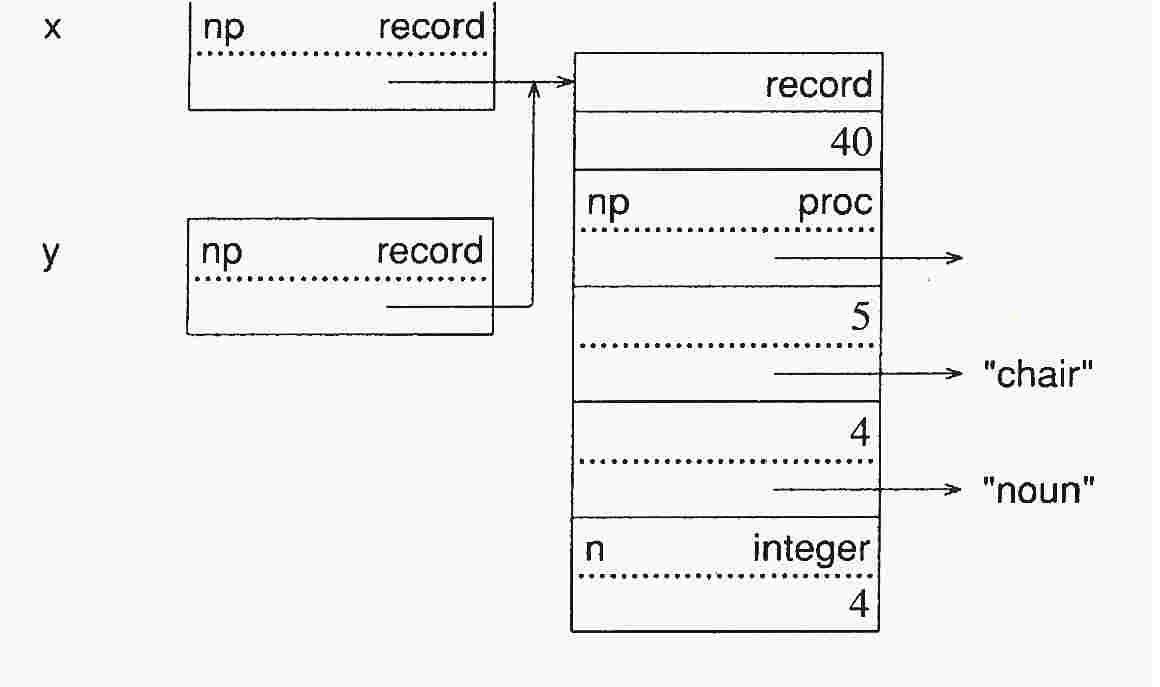
\includegraphics[width=3.9543in,height=2.2937in]{ib-img/ib-img090.jpg} 
\begin{picture}(300,190)(-20,0)
\put(140,128){\blkbox{record}{40}}
\put(140,112){\wordbox{\textit{id}}}
\put(140,96){\wordboxptr{50}{record-constructor}}
\put(140,64){\dvboxptr{5}{}{50}{\texttt{"chair"}}}
\put(140,32){\dvboxptr{4}{}{50}{\texttt{"noun"}}}
\put(140,0){\dvbox{integer}{n}{4}}
\put(0,80){\dvbox{record}{np}{}}
\put(0,80){\tlboxlabel{\texttt{y}{\hspace{20pt}}}}
\put(0,80){\ruptr{40}{64}}
\put(0,144){\tlboxlabel{\texttt{x}{\hspace{20pt}}}}
\put(0,144){\dvboxptr{record}{np}{60}{}}
\end{picture}

Suppose that the descriptor containing the value of x is processed
during the location phase before the descriptor containing the value
of y. This descriptor is identified as pointing to a block in the
allocated block region by virtue of the p flag in its d-word and an
address range check on the value of its v-word. The back chain is
established by setting the title word of the block to point to the
descriptor and setting the v-word of the descriptor to hold the
previous contents of the title word. The result is

%--%\ \  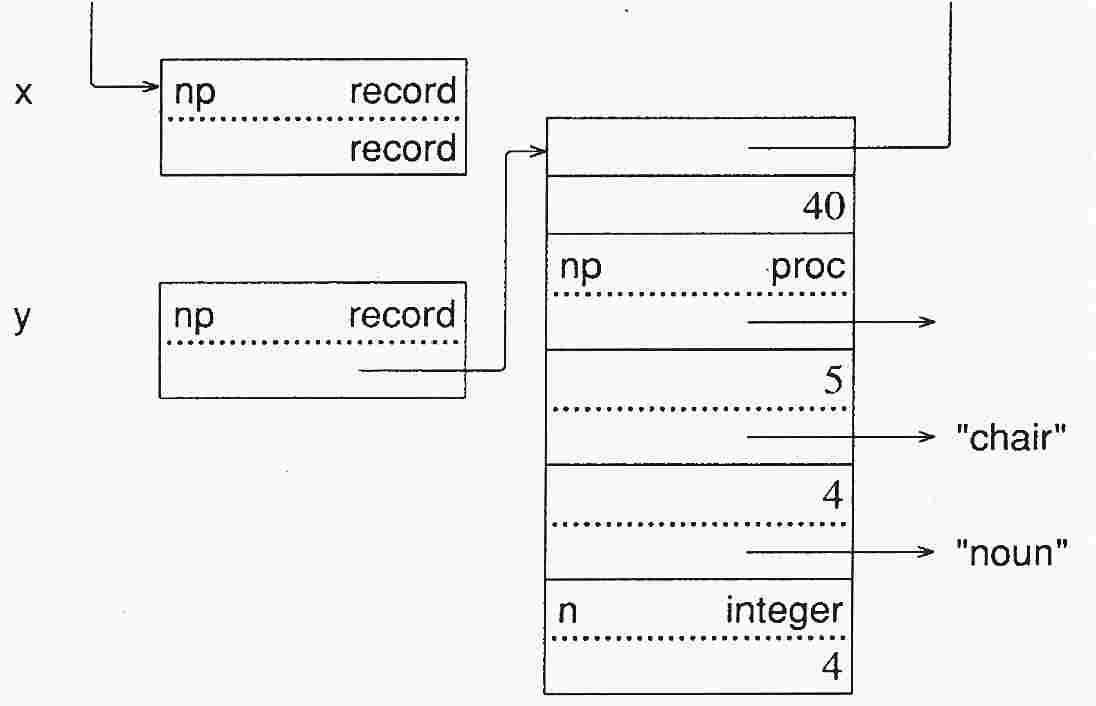
\includegraphics[width=3.7402in,height=2.3571in]{ib-img/ib-img091.jpg} 
\begin{picture}(300,220)(-20,0)
\put(140,128){\blkbox{}{40}}
\put(140,112){\wordbox{\textit{id}}}
\put(140,96){\wordboxptr{50}{record-constructor}}
\put(140,64){\dvboxptr{5}{}{50}{\texttt{"chair"}}}
\put(140,32){\dvboxptr{4}{}{50}{\texttt{"noun"}}}
\put(140,0){\dvbox{integer}{n}{4}}
\put(0,80){\dvbox{record}{np}{}}
\put(0,80){\tlboxlabel{\texttt{y}{\hspace{20pt}}}}
\put(0,144){\tlboxlabel{\texttt{x}{\hspace{20pt}}}}
\put(0,144){\dvbox{record}{np}{record}{}}
\put(80,88){\line(1,0){40}}
\put(120,88){\line(0,1){66}}
\put(120,154){\vector(1,0){20}}
\put(220,154){\line(1,0){60}}
\put(280,154){\line(0,1){40}}
\put(280,194){\line(-1,0){300}}
\put(-20,194){\line(0,-1){24}}
\put(-20,170){\vector(1,0){20}}
\end{picture}

The title word of the block now points to the descriptor that
previously pointed to the block. This change is reversible, and prior
to the completion of the garbage collection process the previous
relationship is restored. A crucial but somewhat subtle aspect of the
change is that it is now possible to tell that the block has been
marked. The numerical magnitude of the value of its title word is
greater than that of any type code, since all descriptors in the
run-time system are at memory locations whose addresses are larger
than the largest type code.

The descriptors in the record block now are processed in the same way
as descriptors in the basis. In order to do this, it is necessary to
know where descriptors are located in the block. Since blocks in the
allocated block region are organized so that all descriptors follow
all non-descriptor data, it is only necessary to know where the first
descriptor is and how large the block is. These values are determined
using two arrays that have entries for each type code.

The first array, \texttt{bsizes}, provides the information that is
needed to determine block sizes. There are three kinds of entries. An
entry of -1 indicates a type for which there is no block or for which
the blocks are not in the allocated block region. Examples are
\texttt{T\_Null} and \texttt{T\_Coexpr}. An entry of 0 indicates that
the size of the block follows the block title. This is the case for
records. Any other entry is the actual size of the block in bytes. For
example, the entry in \texttt{bsizes} for \texttt{T\_List} is 24 on a
32-bit computer.

The second array, \texttt{firstd}, is used to determine the byte
offset of the first descriptor in the block. As with \texttt{bsizes},
a value of -1 indicates a type for which there are no associated
blocks in the allocated block region.  A value of 0 indicates that
there are no descriptors in the block. Examples are \texttt{T\_Cset}
and \texttt{T\_Real}.  For \texttt{T\_Record}, the entry is 8 for
32-bit computers, indicating that the first descriptor is at an offset
of 8 bytes (2 words) from the beginning of the block. See Sec. 4.2.

Extra information is required to handle blocks that contain block
pointers.  It is necessary to know the location of pointers within the
block. Two further arrays contain this information.  The first array,
\texttt{firstp}, contains the offset in bytes from the start of the
block to the first block pointer. There are three kinds of entry. An
entry of -1 indicates a type for which there are no allocated
blocks. A value of 0 means that there are no block pointers. Any other
value is the offset in bytes of the first block pointer.  The second
array, \texttt{ptrno} contains the number of block pointers in the
block. As with \texttt{firstp}, an entry of -1 denotes a type for
which there are no allocated blocks.  0 means that the rest of the
block contains block pointers and a positive value indicates that there
are exactly that many block pointers.

The constraint that this design places on the implementation is that
all the block pointers must be contiguous within a block and (since
the descriptors must be at the end) before any descriptors. Any block
that may have a variable number of block pointers must have no
descriptors and the pointers must be located at the end of the block.

There is only one block pointer in a record, which points to the
record constructor (of type \texttt{proc}). The result after
processing the record block is that the record constructor block's
back chain points to the block pointer in the record block (the
record constructor block structure is not shown in detail).
 
\begin{picture}(300,220)(-20,0)
\put(140,128){\blkbox{}{40}}
\put(140,112){\wordbox{\textit{id}}}
\put(140,96){\wordbox{proc}}
\put(320,96){\wordbox{}}
\put(320,96){\downetc}
\put(320,110){\makebox(100,16){record-constructor}}
\put(346,104){\vector(-1,0){106}}
\put(140,64){\dvboxptr{5}{}{40}{\texttt{"chair"}}}
\put(140,32){\dvboxptr{4}{}{40}{\texttt{"noun"}}}
\put(140,0){\dvbox{integer}{n}{4}}
\put(0,80){\dvbox{record}{np}{}}
\put(0,80){\tlboxlabel{\texttt{y}{\hspace{20pt}}}}
\put(0,144){\tlboxlabel{\texttt{x}{\hspace{20pt}}}}
\put(0,144){\dvbox{record}{np}{record}{}}
\put(80,88){\line(1,0){40}}
\put(120,88){\line(0,1){66}}
\put(120,154){\vector(1,0){20}}
\put(220,154){\line(1,0){60}}
\put(280,154){\line(0,1){40}}
\put(280,194){\line(-1,0){300}}
\put(-20,194){\line(0,-1){24}}
\put(-20,170){\vector(1,0){20}}
\end{picture}

For the previous example, after the block pointers and descriptors in
the record block are processed, the location phase continues. When the
descriptor that contains the value of y is processed, it is added to
the back chain by again exchanging the contents of its v-word with the
contents of the title of the block. As a result, the title of the
block points to the descriptor for the value of y and its v-word
points to the descriptor for the value of x:

%--%\ \  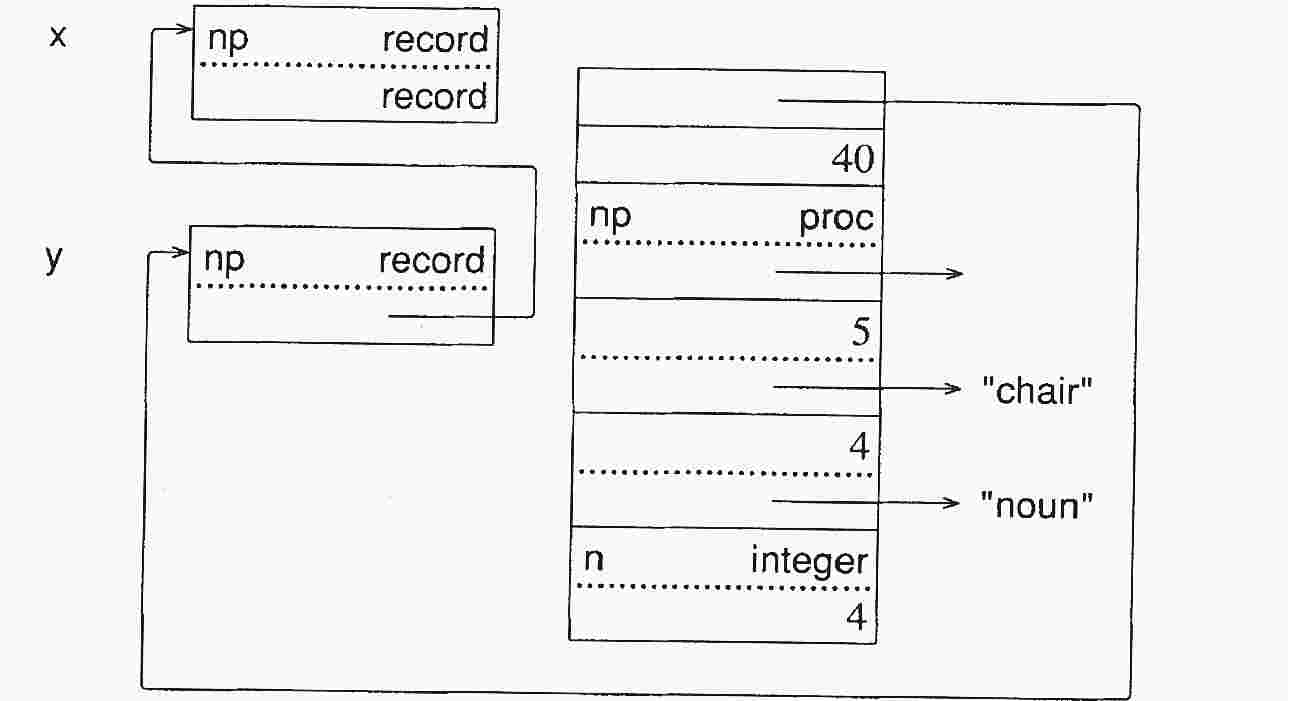
\includegraphics[width=4.3811in,height=2.3402in]{ib-img/ib-img092.jpg} 
\begin{picture}(300,220)(-20,-20)
\put(140,128){\blkbox{}{40}}
\put(140,112){\wordbox{\textit{id}}}
\put(140,96){\wordbox{proc}}
\put(320,96){\wordbox{}}
\put(320,96){\downetc}
\put(320,110){\makebox(100,16){record-constructor}}
\put(346,104){\vector(-1,0){106}}
\put(140,64){\dvboxptr{5}{}{40}{\texttt{"chair"}}}
\put(140,32){\dvboxptr{4}{}{40}{\texttt{"noun"}}}
\put(140,0){\dvbox{integer}{n}{4}}
\put(0,80){\dvbox{record}{np}{}}
\put(0,80){\tlboxlabel{\texttt{y}{\hspace{20pt}}}}
\put(0,144){\tlboxlabel{\texttt{x}{\hspace{20pt}}}}
\put(0,144){\dvbox{record}{np}{record}{}}
\put(80,88){\line(1,0){40}}
\put(120,88){\line(0,1){40}}
\put(120,128){\line(-1,0){140}}
\put(-20,128){\line(0,1){42}}
\put(220,154){\line(1,0){95}}
\put(315,154){\line(0,-1){48}}
\put(315,104){\oval(4,4)[r]}
\put(315,102){\line(0,-1){118}}
\put(315,-16){\line(-1,0){335}}
\put(-20,-16){\line(0,1){120}}
\put(-20,104){\vector(1,0){20}}
\put(-20,170){\vector(1,0){20}}
\end{picture}

Since the title of the block that y points to is marked, the
descriptors in it are not processed. This prevents descriptors from
being processed twice and also prevents the marking phase from looping
in case there are pointer loops among blocks.

If a variable descriptor is encountered when processing descriptors
whose d-words contain p flags, the value the variable points to
belongs to one of the following categories:

\liststyleLxiv
\begin{itemize}
\item 
\ trapped-variable block
\item 
\ global or static identifier
\item 
\ argument or local identifier
%\item 
%\ descriptor in a structure
\end{itemize}

% Remove the Icon V6 special treatment of descriptors pointing within structures 
A trapped variable, indicated by a t flag in its v-word, points to a
block and is processed like any other descriptor that points to a
block. The values of global and static identifiers are in the basis
and are processed separately. The values of arguments and local
identifiers are on an interpreter stack and are processed when its
co-expression block is processed. %A variable descriptor that points to
%a descriptor in a structure points \textit{within} a block, not to the
%title of a block. This is the only case in which the offset, which is
%contained in the least-significant portion of the d-word of a
%non-trapped-variable descriptor, is nonzero. Consequently, this offset
%is used to distinguish such variables from those in the second and
%third categories.

Continuing the previous example, suppose that a garbage collection is
triggered by evaluation of the expression

%-% {\ttfamily\mdseries
%-% \ \ x.count := read()}
\iconline{\> x.count := read() }

At the beginning of garbage collection, there is a variable descriptor
for the field reference that points to the record block in addition to
the descriptors for the values of x and y. If the values of x and y
are processed first as described previously, the situation when the
variable descriptor is encountered is

%--%\ \  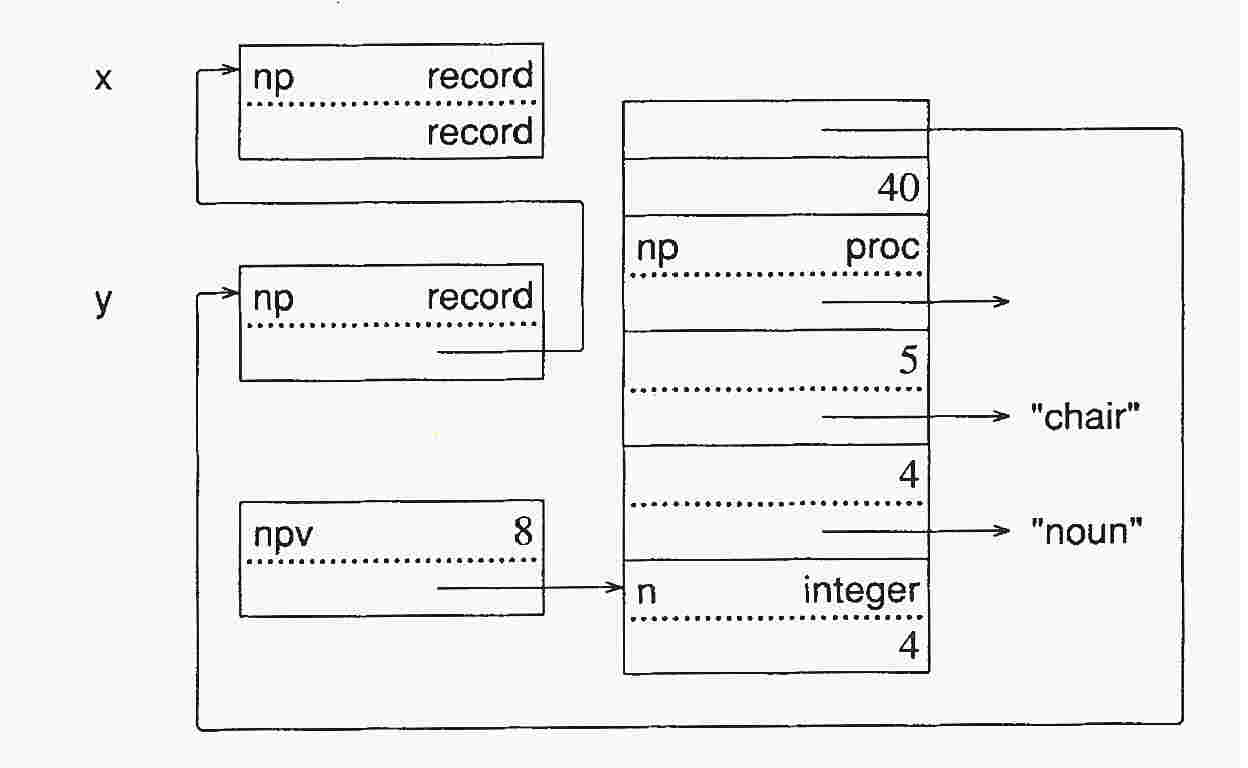
\includegraphics[width=4.1681in,height=2.5654in]{ib-img/ib-img093.jpg} 
\begin{picture}(300,220)(-20,-20)
\put(140,128){\blkbox{}{40}}
\put(140,112){\wordbox{\textit{id}}}
\put(140,96){\wordbox{proc}}
\put(320,96){\wordbox{}}
\put(320,96){\downetc}
\put(320,110){\makebox(100,16){record-constructor}}
\put(346,104){\vector(-1,0){106}}
\put(140,64){\dvboxptr{5}{}{40}{\texttt{"chair"}}}
\put(140,32){\dvboxptr{4}{}{40}{\texttt{"noun"}}}
\put(140,0){\dvbox{integer}{n}{4}}
\put(0,80){\dvbox{record}{np}{}}
\put(0,80){\tlboxlabel{\texttt{y}{\hspace{20pt}}}}
\put(0,144){\tlboxlabel{\texttt{x}{\hspace{20pt}}}}
\put(0,144){\dvbox{record}{np}{record}{}}
\put(0,16){\dvboxptr{8}{npv}{46}{}}
\put(126,24){\line(0,1){128}}
\put(126,152){\vector(1,0){14}}
\multiput(126,24)(4,0){3}{\line(1,0){2}}
\put(136,24){\vector(1,0){4}}
\put(80,88){\line(1,0){40}}
\put(120,88){\line(0,1){40}}
\put(120,128){\line(-1,0){140}}
\put(-20,128){\line(0,1){42}}
\put(220,154){\line(1,0){95}}
\put(315,154){\line(0,-1){48}}
\put(315,104){\oval(4,4)[r]}
\put(315,102){\line(0,-1){118}}
\put(315,-16){\line(-1,0){335}}
\put(-20,-16){\line(0,1){120}}
\put(-20,104){\vector(1,0){20}}
\put(-20,170){\vector(1,0){20}}
\end{picture}

% Convert from V6 garbage collection to V8
Note that the offset in the d-word of the variable descriptor is in
words, not bytes. %The offset, converted to bytes, is added to the
%v-word in the variable descriptor, and this descriptor is linked into
%the back chain.


%--%\ \  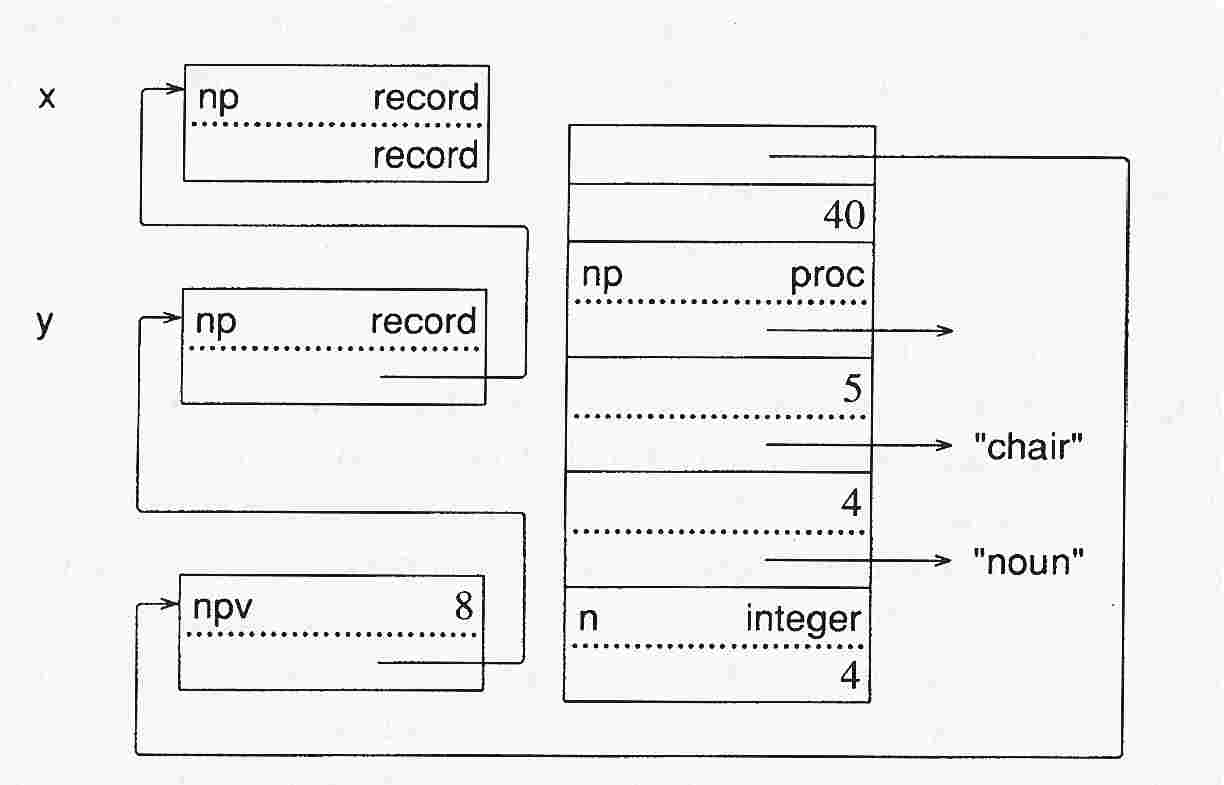
\includegraphics[width=4.1681in,height=2.6217in]{ib-img/ib-img094.jpg} 
\begin{picture}(300,220)(-20,-20)
\put(140,128){\blkbox{}{40}}
\put(140,112){\wordbox{\textit{id}}}
\put(140,96){\wordbox{proc}}
\put(320,96){\wordbox{}}
\put(320,96){\downetc}
\put(320,110){\makebox(100,16){record-constructor}}
\put(346,104){\vector(-1,0){106}}
\put(140,64){\dvboxptr{5}{}{40}{\texttt{"chair"}}}
\put(140,32){\dvboxptr{4}{}{40}{\texttt{"noun"}}}
\put(140,0){\dvbox{integer}{n}{4}}
\put(0,80){\dvbox{record}{np}{}}
\put(0,80){\tlboxlabel{\texttt{y}{\hspace{20pt}}}}
\put(0,144){\tlboxlabel{\texttt{x}{\hspace{20pt}}}}
\put(0,144){\dvbox{record}{np}{record}{}}
\put(0,16){\dvbox{8}{npv}{}}
\put(80,88){\line(1,0){40}}
\put(120,88){\line(0,1){40}}
\put(120,128){\line(-1,0){140}}
\put(-20,128){\line(0,1){42}}
\put(220,154){\line(1,0){95}}
\put(315,154){\line(0,-1){48}}
\put(315,104){\oval(4,4)[r]}
\put(315,102){\line(0,-1){118}}
\put(315,-16){\line(-1,0){335}}
\put(-20,-16){\line(0,1){56}}
\put(-20,170){\vector(1,0){20}}
\put(-20,40){\vector(1,0){20}}
\put(80,24){\line(1,0){40}}
\put(120,24){\line(0,1){40}}
\put(120,64){\line(-1,0){140}}
\put(-20,64){\line(0,1){40}}
\put(-20,104){\vector(1,0){20}}
\end{picture}

When the location phase is complete, the title of each block in the
allocated block region that must be saved points to a chain of all the
descriptors that originally pointed to it. This provides the necessary
information to adjust the v-words of these descriptors to account for
the relocation of the block during the compaction phase. See
Sec. 11.3.3.

If a descriptor that points to a co-expression block is encountered
during the location phase, the title of the co-expression block is
marked and the descriptors in the co-expression block are processed in
a fashion similar to that for blocks in the allocated block
region. Since co-expression blocks are never moved, it is not
necessary to keep track of descriptors that point to them. To mark the
title, it is sufficient to change it to a value that is larger than
any type code.

The activator of the co-expression (if any) is processed like any
other co-expression block. Similarly, the refresh block that is
pointed to from the co-expression block must be processed like any
other block. The rest of the descriptors associated with a
co-expression are in its interpreter stack.

Here the situation is more complicated than it is with blocks in the
allocated block region, since interpreter stacks contain frame markers
in addition to descriptors. Despite this, all the descriptors, and
only the descriptors, on an interpreter stack must be processed.

Interpreter stacks are processed by the routine \texttt{sweep()},
which starts at \texttt{sp} for the stack and works toward the stack
base. Descriptors are processed until the next frame marker is
encountered, at which point, depending on the type of the frame, the
marker is skipped and new frame pointers are set up from it.

The routine for marking blocks is

%-% {\ttfamily\mdseries
%-% static void markblock(dp)
%-% }
%-% 
%-% {\ttfamily\mdseries
%-% dptr dp;
%-% }
%-% 
%-% {\ttfamily\mdseries
%-% \ \ \ \{
%-% }
%-% 
%-% {\ttfamily\mdseries
%-% \ \ \ register dptr dp1;
%-% }
%-% 
%-% {\ttfamily\mdseries
%-% \ \ \ register char *block, *endblock;
%-% }
%-% 
%-% {\ttfamily\mdseries
%-% \ \ \ word type, fdesc;
%-% }
%-% 
%-% {\ttfamily\mdseries
%-% \ \ \ int numptr;
%-% }
%-% 
%-% {\ttfamily\mdseries
%-% \ \ \ register union block **ptr, **lastptr;
%-% }
%-% 
%-% 
%-% \bigskip
%-% 
%-% {\ttfamily\mdseries
%-% \ \ \ if (Var(*dp)) \{
%-% }
%-% 
%-% {\ttfamily\mdseries
%-% \ \ \ \ \ \ \ if (dp-{\textgreater}dword \& F\_Typecode) \{
%-% }
%-% 
%-% {\ttfamily\mdseries
%-% \ \ \ \ \ \ \ \ \ \ switch (Type(*dp)) \{
%-% }
%-% 
%-% {\ttfamily\mdseries
%-% \ \ \ \ \ \ \ \ \ \ \ \ \ case T\_Kywdint:
%-% }
%-% 
%-% {\ttfamily\mdseries
%-% \ \ \ \ \ \ \ \ \ \ \ \ \ case T\_Kywdpos:
%-% }
%-% 
%-% {\ttfamily\mdseries
%-% \ \ \ \ \ \ \ \ \ \ \ \ \ case T\_Kywdsubj:
%-% }
%-% 
%-% {\ttfamily\mdseries
%-% \ \ \ \ \ \ \ \ \ \ \ \ \ \ \ \ /*
%-% }
%-% 
%-% {\ttfamily\mdseries
%-% \ \ \ \ \ \ \ \ \ \ \ \ \ \ \ \ \ * descriptor points to a keyword, not a block.
%-% }
%-% 
%-% {\ttfamily\mdseries
%-% \ \ \ \ \ \ \ \ \ \ \ \ \ \ \ \ \ */
%-% }
%-% 
%-% {\ttfamily\mdseries
%-% \ \ \ \ \ \ \ \ \ \ \ \ \ \ \ \ return;
%-% }
%-% 
%-% {\ttfamily\mdseries
%-% \ \ \ \ \ \ \ \ \ \ \ \ \ \}
%-% }
%-% 
%-% {\ttfamily\mdseries
%-% \ \ \ \ \ \ \ \ \ \ \}
%-% }
%-% 
%-% {\ttfamily\mdseries
%-% \ \ \ \ \ \ \ else if (Offset(*dp) == 0) \{
%-% }
%-% 
%-% {\ttfamily\mdseries
%-% \ \ \ \ \ \ \ \ \ \ /*
%-% }
%-% 
%-% {\ttfamily\mdseries
%-% \ \ \ \ \ \ \ \ \ \ \ * A simple variable not residing in a block. \ \ \ \ \ \ }
%-% 
%-% {\ttfamily\mdseries
%-% \ \ \ \ \ \ \ \ \ \ \ */
%-% }
%-% 
%-% {\ttfamily\mdseries
%-% \ \ \ \ \ \ \ \ \ \ return;
%-% }
%-% 
%-% {\ttfamily\mdseries
%-% \ \ \ \ \ \ \ \ \ \ \}
%-% }
%-% 
%-% {\ttfamily\mdseries
%-% \ \ \ \ \ \ \}
%-% }
%-% 
%-% 
%-% \bigskip
%-% 
%-% {\ttfamily\mdseries
%-% \ \ \ /*
%-% }
%-% 
%-% {\ttfamily\mdseries
%-% \ \ \ \ * Get the block to which dp points.
%-% }
%-% 
%-% {\ttfamily\mdseries
%-% \ \ \ \ */
%-% }
%-% 
%-% {\ttfamily\mdseries
%-% \ \ \ block = (char *)BlkLoc(*dp);
%-% }
%-% 
%-% 
%-% \bigskip
%-% 
%-% {\ttfamily\mdseries
%-% \ \ \ if (InRange(blkbase,block,blkfree)) \{
%-% }
%-% 
%-% {\ttfamily\mdseries
%-% \ \ \ \ \ \ type = BlkType(block);
%-% }
%-% 
%-% {\ttfamily\mdseries
%-% \ \ \ \ \ \ if ((uword)type {\textless}= MaxType) \{
%-% }
%-% 
%-% 
%-% \bigskip
%-% 
%-% {\ttfamily\mdseries
%-% \ \ \ \ \ \ \ \ \ /*
%-% }
%-% 
%-% {\ttfamily\mdseries
%-% \ \ \ \ \ \ \ \ \ \ * The type is valid, which indicates that this block}
%-% 
%-% {\ttfamily\mdseries
%-% \ \ \ \ \ \ \ \ \ \ * \ has not been marked. \ Point endblock to the byte}
%-% 
%-% {\ttfamily\mdseries
%-% \ \ \ \ \ \ \ \ \ \ * \ past the end of the block.
%-% }
%-% 
%-% {\ttfamily\mdseries
%-% \ \ \ \ \ \ \ \ \ \ */
%-% }
%-% 
%-% {\ttfamily\mdseries
%-% \ \ \ \ \ \ \ \ \ endblock = block + BlkSize(block);
%-% }
%-% 
%-% {\ttfamily\mdseries
%-% \ \ \ \ \ \ \ \ \ \}
%-% }
%-% 
%-% 
%-% \bigskip
%-% 
%-% {\ttfamily\mdseries
%-% \ \ \ \ \ \ /*
%-% }
%-% 
%-% {\ttfamily\mdseries
%-% \ \ \ \ \ \ \ * Add dp to the back chain for the block and point the
%-% }
%-% 
%-% {\ttfamily\mdseries
%-% \ \ \ \ \ \ \ * \ block (via the type field) to dp.vword.
%-% }
%-% 
%-% {\ttfamily\mdseries
%-% \ \ \ \ \ \ \ */
%-% }
%-% 
%-% {\ttfamily\mdseries
%-% \ \ \ \ \ \ BlkLoc(*dp) = (union block *)type;
%-% }
%-% 
%-% {\ttfamily\mdseries
%-% \ \ \ \ \ \ BlkType(block) = (uword)\&BlkLoc(*dp);}
%-% 
%-% \bigskip
%-% 
%-% {\ttfamily\mdseries
%-% \ \ \ \ \ \ if ((uword)type {\textless}= MaxType) \{
%-% }
%-% 
%-% {\ttfamily\mdseries
%-% \ \ \ \ \ \ \ \ \ /*
%-% }
%-% 
%-% {\ttfamily\mdseries
%-% \ \ \ \ \ \ \ \ \ \ * The block was not marked; process pointers and
%-% }
%-% 
%-% {\ttfamily\mdseries
%-% \ \ \ \ \ \ \ \ \ \ * \ descriptors within the block.
%-% }
%-% 
%-% {\ttfamily\mdseries
%-% \ \ \ \ \ \ \ \ \ \ */
%-% }
%-% 
%-% {\ttfamily\mdseries
%-% \ \ \ \ \ \ \ \ \ if ((fdesc = firstp[type]) {\textgreater} 0) \{
%-% }
%-% 
%-% {\ttfamily\mdseries
%-% \ \ \ \ \ \ \ \ \ \ \ \ /*
%-% }
%-% 
%-% {\ttfamily\mdseries
%-% \ \ \ \ \ \ \ \ \ \ \ \ \ * The block contains pointers; mark each pointer.
%-% }
%-% 
%-% {\ttfamily\mdseries
%-% \ \ \ \ \ \ \ \ \ \ \ \ \ */
%-% }
%-% 
%-% {\ttfamily\mdseries
%-% \ \ \ \ \ \ \ \ \ \ \ \ ptr = (union block **)(block + fdesc);
%-% }
%-% 
%-% {\ttfamily\mdseries
%-% \ \ \ \ \ \ \ \ \ \ \ \ numptr = ptrno[type];
%-% }
%-% 
%-% {\ttfamily\mdseries
%-% \ \ \ \ \ \ \ \ \ \ \ \ if (numptr {\textgreater} 0)
%-% }
%-% 
%-% {\ttfamily\mdseries
%-% \ \ \ \ \ \ \ \ \ \ \ \ \ \ \ lastptr = ptr + numptr;
%-% }
%-% 
%-% {\ttfamily\mdseries
%-% \ \ \ \ \ \ \ \ \ \ \ \ else
%-% }
%-% 
%-% {\ttfamily\mdseries
%-% \ \ \ \ \ \ \ \ \ \ \ \ \ \ \ lastptr = (union block **)endblock;
%-% }
%-% 
%-% {\ttfamily\mdseries
%-% \ \ \ \ \ \ \ \ \ \ \ \ for (; ptr {\textless} lastptr; ptr++)
%-% }
%-% 
%-% {\ttfamily\mdseries
%-% \ \ \ \ \ \ \ \ \ \ \ \ \ \ \ if (*ptr != NULL)
%-% }
%-% 
%-% {\ttfamily\mdseries
%-% \ \ \ \ \ \ \ \ \ \ \ \ \ \ \ \ \ \ markptr(ptr);
%-% }
%-% 
%-% {\ttfamily\mdseries
%-% \ \ \ \ \ \ \ \ \ \ \ \ \}
%-% }
%-% 
%-% {\ttfamily\mdseries
%-% \ \ \ \ \ \ \ \ \ if ((fdesc = firstd[type]) {\textgreater} 0)
%-% }
%-% 
%-% {\ttfamily\mdseries
%-% \ \ \ \ \ \ \ \ \ \ \ \ /*
%-% }
%-% 
%-% {\ttfamily\mdseries
%-% \ \ \ \ \ \ \ \ \ \ \ \ \ * The block contains descriptors; mark each one. }
%-% 
%-% {\ttfamily\mdseries
%-% \ \ \ \ \ \ \ \ \ \ \ \ \ */
%-% }
%-% 
%-% {\ttfamily\mdseries
%-% \ \ \ \ \ \ \ \ \ \ \ \ for (dp1 = (dptr)(block + fdesc);
%-% }
%-% 
%-% {\ttfamily\mdseries
%-% \ \ \ \ \ \ \ \ \ \ \ \ \ \ \ \ \ (char *)dp1 {\textless} endblock; dp1++) \{
%-% }
%-% 
%-% {\ttfamily\mdseries
%-% \ \ \ \ \ \ \ \ \ \ \ \ \ \ \ if (Qual(*dp1))
%-% }
%-% 
%-% {\ttfamily\mdseries
%-% \ \ \ \ \ \ \ \ \ \ \ \ \ \ \ \ \ \ postqual(dp1);
%-% }
%-% 
%-% {\ttfamily\mdseries
%-% \ \ \ \ \ \ \ \ \ \ \ \ \ \ \ else if (Pointer(*dp1))
%-% }
%-% 
%-% {\ttfamily\mdseries
%-% \ \ \ \ \ \ \ \ \ \ \ \ \ \ \ \ \ \ markblock(dp1);
%-% }
%-% 
%-% {\ttfamily\mdseries
%-% \ \ \ \ \ \ \ \ \ \ \ \ \ \ \ \}
%-% }
%-% 
%-% {\ttfamily\mdseries
%-% \ \ \ \ \ \ \ \ \ \}
%-% }
%-% 
%-% {\ttfamily\mdseries
%-% \ \ \ \ \ \ \} }
%-% 
%-% 
%-% \bigskip
%-% 
%-% {\ttfamily\mdseries
%-% \ \ \ else if ((unsigned int)BlkType(block) == T\_Coexpr) \{
%-% }
%-% 
%-% {\ttfamily\mdseries
%-% \ \ \ \ \ \ struct b\_coexpr *cp;
%-% }
%-% 
%-% {\ttfamily\mdseries
%-% \ \ \ \ \ \ struct astkblk *abp;
%-% }
%-% 
%-% {\ttfamily\mdseries
%-% \ \ \ \ \ \ int i;
%-% }
%-% 
%-% {\ttfamily\mdseries
%-% \ \ \ \ \ \ struct descrip adesc;
%-% }
%-% 
%-% 
%-% \bigskip
%-% 
%-% {\ttfamily\mdseries
%-% \ \ \ \ \ \ /*
%-% }
%-% 
%-% {\ttfamily\mdseries
%-% \ \ \ \ \ \ \ * dp points to a co-expression block that has not been
%-% }
%-% 
%-% {\ttfamily\mdseries
%-% \ \ \ \ \ \ \ * \ marked. Point the block to dp. Sweep the interpreter
%-% }
%-% 
%-% {\ttfamily\mdseries
%-% \ \ \ \ \ \ \ * \ stack in the block. \ Then mark the block for the
%-% }
%-% 
%-% {\ttfamily\mdseries
%-% \ \ \ \ \ \ \ * \ activating co-expression and the refresh block.
%-% }
%-% 
%-% {\ttfamily\mdseries
%-% \ \ \ \ \ \ \ */
%-% }
%-% 
%-% {\ttfamily\mdseries
%-% \ \ \ \ \ \ BlkType(block) = (uword)dp;
%-% }
%-% 
%-% {\ttfamily\mdseries
%-% \ \ \ \ \ \ sweep((struct b\_coexpr *)block);
%-% }
%-% 
%-% 
%-% \bigskip
%-% 
%-% {\ttfamily\mdseries
%-% \ \ \ \ \ \ /*
%-% }
%-% 
%-% {\ttfamily\mdseries
%-% \ \ \ \ \ \ \ * Mark the activators of this co-expression. \ \ The
%-% }
%-% 
%-% {\ttfamily\mdseries
%-% \ \ \ \ \ \ \ * \ activators are stored as a list of addresses, but}
%-% 
%-% {\ttfamily\mdseries
%-% \ \ \ \ \ \ \ * \ markblock requires the address of a descriptor. \ To}
%-% 
%-% {\ttfamily\mdseries
%-% \ \ \ \ \ \ \ * \ accommodate markblock, the dummy descriptor adesc is}
%-% 
%-% {\ttfamily\mdseries
%-% \ \ \ \ \ \ \ * \ filled in with each activator address in turn and then}
%-% 
%-% {\ttfamily\mdseries
%-% \ \ \ \ \ \ \ * \ marked. \ Since co-expressions and the descriptors that}
%-% 
%-% {\ttfamily\mdseries
%-% \ \ \ \ \ \ \ * \ reference them don't participate in the back-chaining}
%-% 
%-% {\ttfamily\mdseries
%-% \ \ \ \ \ \ \ * \ scheme, it's ok to reuse the descriptor in this manner.
%-% }
%-% 
%-% {\ttfamily\mdseries
%-% \ \ \ \ \ \ \ */
%-% }
%-% 
%-% {\ttfamily\mdseries
%-% \ \ \ \ \ \ cp = (struct b\_coexpr *)block;
%-% \ \ \ \ \ \ \ \ \ \ \ \ \ \ \ \ \ \ \ \ \ \ \ \ \ \ \ \ \ \ \ \ \ \ \ \ \ \ \ \ \ \ \ }
%-% 
%-% {\ttfamily\mdseries
%-% \ \ \ \ \ \ adesc.dword = D\_Coexpr;
%-% }
%-% 
%-% {\ttfamily\mdseries
%-% \ \ \ \ \ \ for (abp = cp-{\textgreater}es\_actstk; abp!=NULL; abp = abp-{\textgreater}astk\_nxt) \{
%-% }
%-% 
%-% {\ttfamily\mdseries
%-% \ \ \ \ \ \ \ \ \ for (i = 1; i {\textless}= abp-{\textgreater}nactivators; i++) \{
%-% }
%-% 
%-% {\ttfamily\mdseries
%-% \ \ \ \ \ \ \ \ \ \ \ \ BlkLoc(adesc) =}
%-% 
%-% {\ttfamily\mdseries
%-% \ \ \ \ \ \ \ \ \ \ \ \ \ \ \ (union block *)abp-{\textgreater}arec[i-1].activator;}
%-% 
%-% {\ttfamily\mdseries
%-% \ \ \ \ \ \ \ \ \ \ \ \ markblock(\&adesc);
%-% }
%-% 
%-% {\ttfamily\mdseries
%-% \ \ \ \ \ \ \ \ \ \ \ \ \}
%-% }
%-% 
%-% {\ttfamily\mdseries
%-% \ \ \ \ \ \ \ \ \ \}
%-% }
%-% 
%-% {\ttfamily\mdseries
%-% \ \ \ \ \ \ if(BlkLoc(cp-{\textgreater}freshblk) != NULL)
%-% }
%-% 
%-% {\ttfamily\mdseries
%-% \ \ \ \ \ \ \ \ \ markblock(\&((struct b\_coexpr *)block)-{\textgreater}freshblk);
%-% }
%-% 
%-% {\ttfamily\mdseries
%-% \ \ \ \ \ \ \}}
%-% 
%-% {\ttfamily\mdseries
%-% \ \ \ else \{}
%-% 
%-% {\ttfamily\mdseries
%-% \ \ \ \ \ \ /* {\dots} code for blocks found in other regions */}
%-% 
%-% {\ttfamily\mdseries
%-% \ \ \ \ \ \ \}}
%-% 
%-% {\ttfamily\mdseries
%-% \ \ \ \}}
\goodbreak
\iconcode{
static void markblock(dp)\\
dptr dp;\\
\>\{\\
\>register dptr dp1;\\
\>register char *block, *endblock;\\
\>word type, fdesc;\\
\>int numptr;\\
\>register union block **ptr, **lastptr;\\
\\
\>if (Var(*dp)) \{\\
\>\>\ if (dp->dword \& F\_Typecode) \{\\
\>\>\>\ switch (Type(*dp)) \{\\
\>\>\>\>\ case T\_Kywdint:\\
\>\>\>\>\ case T\_Kywdpos:\\
\>\>\>\>\ case T\_Kywdsubj:\\
\>\>\>\>\>\ /*\\
\>\>\>\>\>\ \ * descriptor points to a keyword, not a block.\\
\>\>\>\>\>\ \ */\\
\>\>\>\>\>\ return;\\
\>\>\>\>\ \}\\
\>\>\>\ \}\\
\>\>\ else if (Offset(*dp) == 0) \{\\
\>\>\>\ /*\\
\>\>\>\ \ * A simple variable not residing in a block.\\
\>\>\>\ \ */\\
\>\>\>\ return;\\
\>\>\>\ \}\\
\>\>\}\\
\\
\>/*\\
\>\ * Get the block to which dp points.\\
\>\ */\\
\>block = (char *)BlkLoc(*dp);\\
\\
\>if (InRange(blkbase,block,blkfree)) \{\\
\>\>type = BlkType(block);\\
\>\>if ((uword)type <= MaxType) \{\\
\\
\>\>\>/*\\
\>\>\>\ * The type is valid, which indicates that this block\\
\>\>\>\ * \ has not been marked. \ Point endblock to the byte\\
\>\>\>\ * \ past the end of the block.\\
\>\>\>\ */\\
\>\>\>endblock = block + BlkSize(block);\\
\>\>\>\}\\
\\
\>\>/*\\
\>\>\ * Add dp to the back chain for the block and point the\\
\>\>\ * \ block (via the type field) to dp.vword.\\
\>\>\ */\\
\>\>BlkLoc(*dp) = (union block *)type;\\
\>\>BlkType(block) = (uword)\&BlkLoc(*dp);\\
\\
\>\>if ((uword)type <= MaxType) \{\\
\>\>\>/*\\
\>\>\>\ * The block was not marked; process pointers and\\
\>\>\>\ * \ descriptors within the block.\\
\>\>\>\ */\\
\>\>\>if ((fdesc = firstp[type]) > 0) \{\\
\>\>\>\>/*\\
\>\>\>\>\ * The block contains pointers; mark each pointer.\\
\>\>\>\>\ */\\
\>\>\>\>ptr = (union block **)(block + fdesc);\\
\>\>\>\>numptr = ptrno[type];\\
\>\>\>\>if (numptr > 0)\\
\>\>\>\>\>lastptr = ptr + numptr;\\
\>\>\>\>else\\
\>\>\>\>\>lastptr = (union block **)endblock;\\
\>\>\>\>for (; ptr < lastptr; ptr++)\\
\>\>\>\>\>if (*ptr != NULL)\\
\>\>\>\>\>\>markptr(ptr);\\
\>\>\>\>\}\\
\>\>\>if ((fdesc = firstd[type]) > 0)\\
\>\>\>\>/*\\
\>\>\>\>\ * The block contains descriptors; mark each one. 
\>\>\>\>\ */\\
\>\>\>\>for (dp1 = (dptr)(block + fdesc);\\
\>\>\>\>\>\ \ (char *)dp1 < endblock; dp1++) \{\\
\>\>\>\>\>if (Qual(*dp1))\\
\>\>\>\>\>\>postqual(dp1);\\
\>\>\>\>\>else if (Pointer(*dp1))\\
\>\>\>\>\>\>markblock(dp1);\\
\>\>\>\>\>\}\\
\>\>\>\}\\
\>\>\}\\
\\
\>else if ((unsigned int)BlkType(block) == T\_Coexpr) \{\\
\>\>struct b\_coexpr *cp;\\
\>\>struct astkblk *abp;\\
\>\>int i;\\
\>\>struct descrip adesc;\\
\\
\>\>/*\\
\>\>\ * dp points to a co-expression block that has not been\\
\>\>\ * \ marked. Point the block to dp. Sweep the interpreter\\
\>\>\ * \ stack in the block. \ Then mark the block for the\\
\>\>\ * \ activating co-expression and the refresh block.\\
\>\>\ */\\
\>\>BlkType(block) = (uword)dp;\\
\>\>sweep((struct b\_coexpr *)block);\\
\\
\>\>/*\\
\>\>\ * Mark the activators of this co-expression. \ \ The\\
\>\>\ * \ activators are stored as a list of addresses, but\\
\>\>\ * \ markblock requires the address of a descriptor. \ To\\
\>\>\ * \ accommodate markblock, the dummy descriptor adesc is\\
\>\>\ * \ filled in with each activator address in turn and then\\
\>\>\ * \ marked. \ Since co-expressions and the descriptors that\\
\>\>\ * \ reference them don't participate in the back-chaining\\
\>\>\ * \ scheme, it's ok to reuse the descriptor in this manner.\\
\>\>\ */\\
\>\>cp = (struct b\_coexpr *)block;\\
\>\>adesc.dword = D\_Coexpr;\\
\>\>for (abp = cp->es\_actstk; abp!=NULL; abp = abp->astk\_nxt) \{\\
\>\>\>for (i = 1; i <= abp->nactivators; i++) \{\\
\>\>\>\>BlkLoc(adesc) =\\
\>\>\>\>\>(union block *)abp->arec[i-1].activator;\\
\>\>\>\>markblock(\&adesc);\\
\>\>\>\>\}\\
\>\>\>\}\\
\>\>if(BlkLoc(cp->freshblk) != NULL)\\
\>\>\>markblock(\&((struct b\_coexpr *)block)->freshblk);\\
\>\>\}\\
\>else \{\\
\>\>/* {\dots} code for blocks found in other regions */\\
\>\>\}\\
\>\}
}

The macro \texttt{BlkType(cp)} produces the type code of the block
pointed to by \texttt{cp}. The macro \texttt{BlkSize(cp)} uses the
array \texttt{bsizes} to determine the size of the block pointed to by
\texttt{cp}.

\subsection[11.3.3 Pointer Adjustment and Compaction]{11.3.3 Pointer Adjustment and Compaction}

\textbf{Strings}. When the location phase is complete, quallist
contains a list pointers to all the qualifiers whose v-words point to
the allocated string region. For example, suppose that the allocated
string region at the beginning of a garbage collection is

\begin{center}
%--%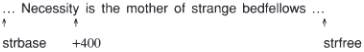
\includegraphics[width=4.3445in,height=0.5626in]{ib-img/ib-img095.png}
\begin{picture}(300,40)
\put(0,30){\dots \texttt{\ Necessity is the mother of strange bedfellows\ } \dots}
\put(0,0){\texttt{strbase}}
\put(0,15){\vector(0,1){10}}
\put(66,15){\vector(0,1){10}}
\put(62,0){+400}
\put(280,15){\vector(0,1){10}}
\put(280,0){\texttt{strfree}}
\end{picture}
\end{center}

\bigskip

Suppose also that the following qualifiers reference the allocated
string region:


%--%\ \  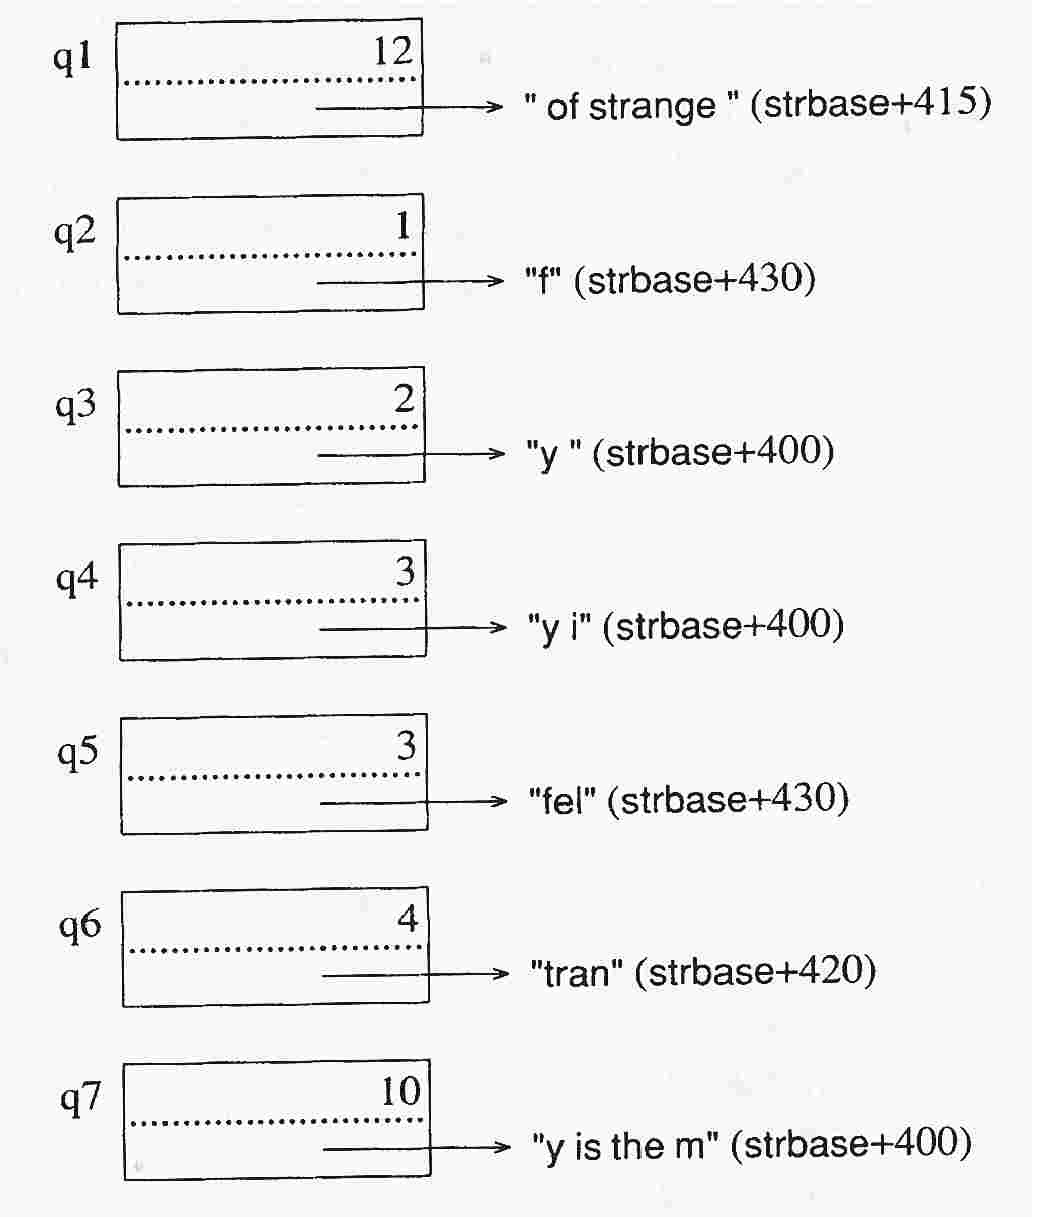
\includegraphics[width=3.5272in,height=4.0638in]{ib-img/ib-img096.jpg}
%
% Pictures are separate to avoid a horrific page break 
\begin{picture}(300,40)(-100,0)
\put(0,0){\dvboxptr{12}{}{40}{\texttt{" of strange " (strbase+415)}}}
\put(0,0){\tlboxlabel{q1}}
\end{picture}

\begin{picture}(300,40)(-100,0)
\put(0,0){\dvboxptr{1}{}{40}{\texttt{"f" (strbase+430)}}}
\put(0,0){\tlboxlabel{q2}}
\end{picture}

\begin{picture}(300,40)(-100,0)
\put(0,0){\dvboxptr{2}{}{40}{\texttt{"y " (strbase+400)}}}
\put(0,0){\tlboxlabel{q3}}
\end{picture}

\begin{picture}(300,40)(-100,0)
\put(0,0){\dvboxptr{3}{}{40}{\texttt{"y i" (strbase+400)}}}
\put(0,0){\tlboxlabel{q4}}
\end{picture}

\begin{picture}(300,40)(-100,0)
\put(0,0){\dvboxptr{3}{}{40}{\texttt{"fel" (strbase+430)}}}
\put(0,0){\tlboxlabel{q5}}
\end{picture}

\begin{picture}(300,40)(-100,0)
\put(0,0){\dvboxptr{4}{}{40}{\texttt{"tran" (strbase+420)}}}
\put(0,0){\tlboxlabel{q6}}
\end{picture}

\begin{picture}(300,40)(-100,0)
\put(0,0){\dvboxptr{10}{}{40}{\texttt{"y is the m" (strbase+400)}}}
\put(0,0){\tlboxlabel{q7}}
\end{picture}

\goodbreak
The pointers to the allocated string region are

\begin{center}
%--%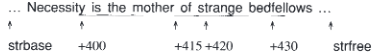
\includegraphics[width=4.0425in,height=0.6374in]{ib-img/ib-img097.png}
\begin{picture}(300,40)
\put(0,36){\dots \texttt{\ Necessity is the mother of strange bedfellows\ } \dots}
\put(0,0){\texttt{strbase}}
\begin{picture}(0,0)(5,0)
\put(66,0){+400}
\put(140,0){+415}
\put(170,0){+420}
\put(226,0){+430}
\end{picture}
\begin{picture}(0,0)(6,0)
\put(0,15){\vector(0,1){10}}
\put(68,15){\vector(0,1){10}}
\put(146,15){\vector(0,1){10}}
\put(168,15){\vector(0,1){10}}
\put(226,15){\vector(0,1){10}}
\put(285,15){\vector(0,1){10}}
\end{picture}
\put(280,0){\texttt{strfree}}
\begin{picture}(0,0)(0,-26)
\thicklines
\put(140,6){\line(1,0){60}}% q1
\put(220,6){\line(1,0){4}}% q2
\put(62,6){\line(1,0){4}}% q3
\put(62,4){\line(1,0){12}}% q4
\put(220,4){\line(1,0){12}}% q5
\put(162,4){\line(1,0){20}}% q6
\put(62,2){\line(1,0){48}}% q7
\end{picture}
\end{picture}
\end{center}

Note that the qualifiers point to overlapping strings.


After the location phase, \texttt{quallist} might contain the
following pointers:


\begin{center}
%--%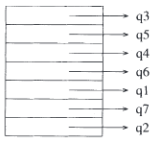
\includegraphics[width=1.389in,height=1.4189in]{ib-img/ib-img098.png}
\begin{picture}(300,120)
\multiput(50,0)(0,16){7}{\wordbox{}{}}
\multiput(125,8)(0,16){7}{\vector(1,0){60}}
\begin{picture}(0,0)(0,-6)
\put(190,0){q2}
\put(190,16){q7}
\put(190,32){q1}
\put(190,48){q6}
\put(190,64){q4}
\put(190,80){q5}
\put(190,96){q3}
\end{picture}
\end{picture}
\end{center}

The order of the pointers in \texttt{quallist} depends on the order in
which the qualifiers are processed: there is no necessary relationship
between the order of the pointers in \texttt{quallist} and the order
of the pointers to the allocated string region.


At the beginning of the pointer-adjustment phase of garbage
collection, the array \texttt{quallist} is sorted in non-decreasing
order by the v-words in qualifiers that are pointed to from
\texttt{quallist}. This allows the pointers to the allocated string
region to be processed in non-decreasing order so that the portions of
the allocated string region that must be saved and compacted can be
determined.


Continuing the previous example, \texttt{quallist} becomes


%--% 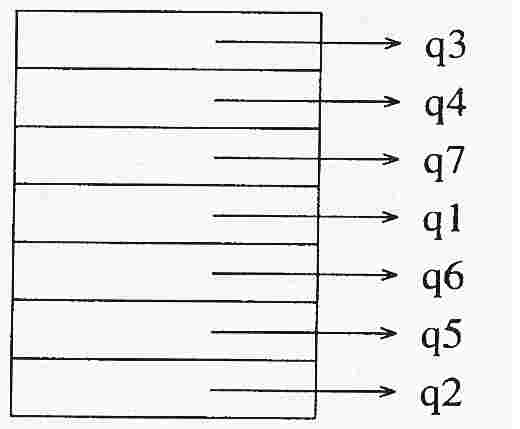
\includegraphics[width=1.8161in,height=1.4319in]{ib-img/ib-img099.jpg} 
\begin{center}
\begin{picture}(300,120)
\multiput(50,0)(0,16){7}{\wordbox{}{}}
\multiput(125,8)(0,16){7}{\vector(1,0){60}}
\begin{picture}(0,0)(0,-6)
\put(190,0){q2}
\put(190,16){q5}
\put(190,32){q6}
\put(190,48){q1}
\put(190,64){q7}
\put(190,80){q4}
\put(190,96){q3}
\end{picture}
\end{picture}
\end{center}


The v-words of the qualifiers in the order of the pointers in
\texttt{quallist} now are

\iconcode{
\>\>\>strbase+400\\
\>\>\>strbase+400\\
\>\>\>strbase+400\\
\>\>\>strbase+415\\
\>\>\>strbase+420\\
\>\>\>strbase+430\\
\>\>\>strbase+430
}

Since qualifiers may reference overlapping strings, care must be taken
to identify contiguous ``clumps'' of characters that may be shared by
qualifiers. The pointers in \texttt{quallist} are processed in
order. Three pointers in the string region are maintained: dest, the
next free destination for a clump of characters to be saved; source,
the start of the next clump; and cend, the end character in the
current clump.

When a qualifier that is pointed to from \texttt{quallist} is
processed, the first question is whether its v-word addresses a
character that is beyond the end of the current clump (since v-words
are processed in numerical order, the address is either in the current
clump or beyond the end of it). If it is in the current clump, cend is
updated, provided the last character of the current qualifier is
beyond cend. If it is not in the current clump, the clump is moved
from source to dest. In either case, the v-word of the current
qualifier is adjusted (dest -source is added to it).

In the previous example, the allocated string region after collection is

\begin{center}
%--%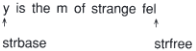
\includegraphics[width=2.3807in,height=0.5193in]{ib-img/strangefel.png}
\begin{picture}(300,40)
\put(0,30){\texttt{y is the m of strange fel}}
\put(0,0){\texttt{strbase}}
\put(0,15){\vector(0,1){10}}
\put(126,15){\vector(0,1){10}}
\put(126,0){\texttt{strfree}}
\end{picture}
\end{center}

and the seven qualifiers that point to it are

%--%\ \  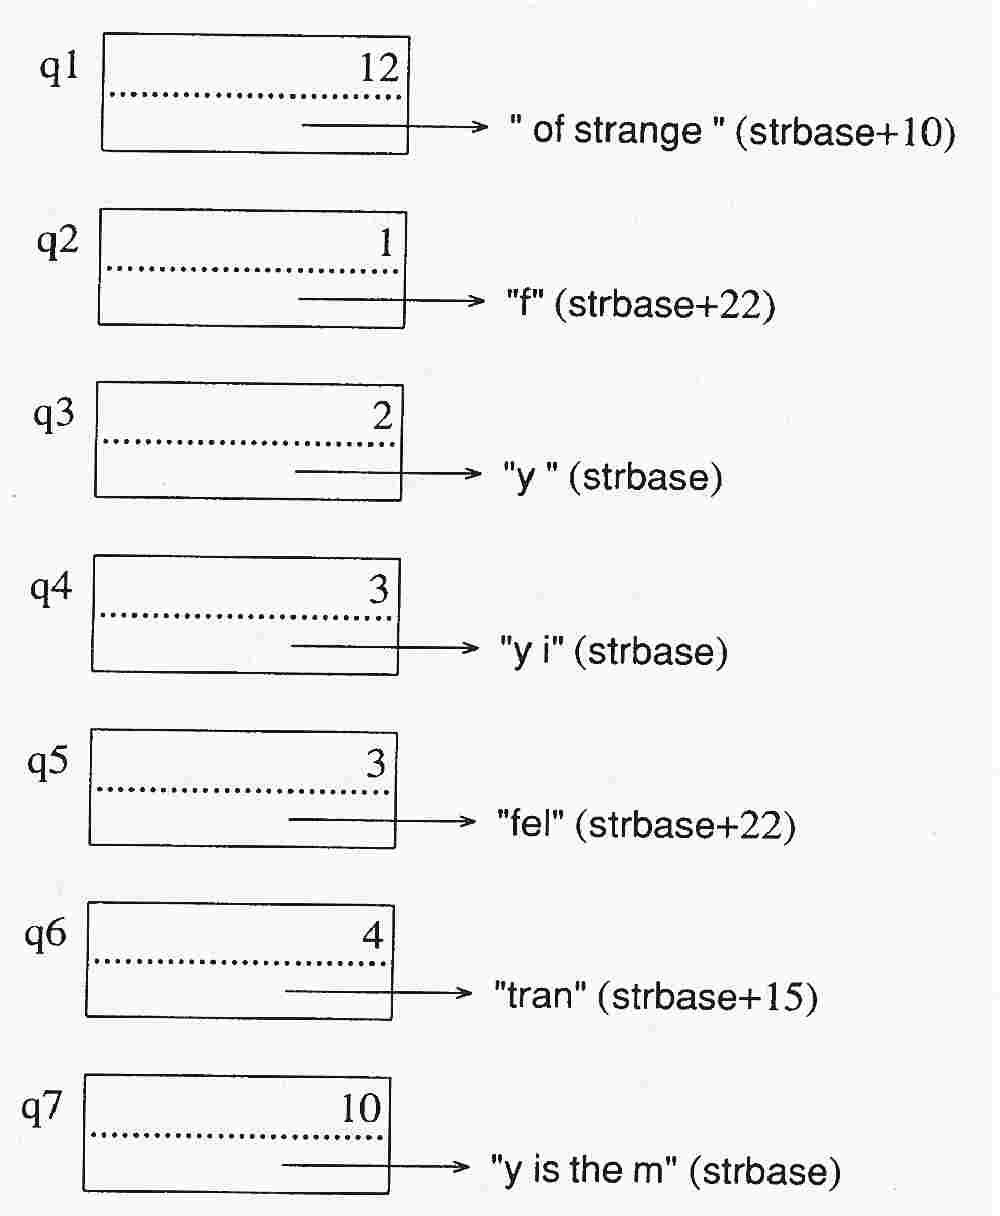
\includegraphics[width=3.4193in,height=4.0602in]{ib-img/ib-img101.jpg} 
%
% Pictures are separate to avoid a horrific page break 
\begin{picture}(300,40)(-100,0)
\put(0,0){\dvboxptr{12}{}{40}{\texttt{" of strange " (strbase+10)}}}
\put(0,0){\tlboxlabel{q1}}
\end{picture}

\begin{picture}(300,40)(-100,0)
\put(0,0){\dvboxptr{1}{}{40}{\texttt{"f" (strbase+22)}}}
\put(0,0){\tlboxlabel{q2}}
\end{picture}

\begin{picture}(300,40)(-100,0)
\put(0,0){\dvboxptr{2}{}{40}{\texttt{"y " (strbase)}}}
\put(0,0){\tlboxlabel{q3}}
\end{picture}

\begin{picture}(300,40)(-100,0)
\put(0,0){\dvboxptr{3}{}{40}{\texttt{"y i" (strbase)}}}
\put(0,0){\tlboxlabel{q4}}
\end{picture}

\begin{picture}(300,40)(-100,0)
\put(0,0){\dvboxptr{3}{}{40}{\texttt{"fel" (strbase+22)}}}
\put(0,0){\tlboxlabel{q5}}
\end{picture}

\begin{picture}(300,40)(-100,0)
\put(0,0){\dvboxptr{4}{}{40}{\texttt{"tran" (strbase+15)}}}
\put(0,0){\tlboxlabel{q6}}
\end{picture}

\begin{picture}(300,40)(-100,0)
\put(0,0){\dvboxptr{10}{}{40}{\texttt{"y is the m" (strbase)}}}
\put(0,0){\tlboxlabel{q7}}
\end{picture}

\goodbreak
The routine for compacting the allocated string region and adjusting pointers to it is

%-% {\ttfamily\mdseries
%-% static void scollect(extra)
%-% }
%-% 
%-% {\ttfamily\mdseries
%-% word extra;
%-% }
%-% 
%-% {\ttfamily\mdseries
%-% \ \ \ \{
%-% }
%-% 
%-% {\ttfamily\mdseries
%-% \ \ \ register char *source, *dest;
%-% }
%-% 
%-% {\ttfamily\mdseries
%-% \ \ \ register dptr *qptr;
%-% }
%-% 
%-% {\ttfamily\mdseries
%-% \ \ \ char *cend;
%-% }
%-% 
%-% {\ttfamily\mdseries
%-% \ \ \ CURTSTATE();
%-% }
%-% 
%-% \bigskip
%-% 
%-% {\ttfamily\mdseries
%-% \ \ \ if (qualfree {\textless}= quallist) \{
%-% }
%-% 
%-% {\ttfamily\mdseries
%-% \ \ \ \ \ \ /*
%-% }
%-% 
%-% {\ttfamily\mdseries
%-% \ \ \ \ \ \ \ * There are no accessible strings. Thus, there are none to}
%-% 
%-% {\ttfamily\mdseries
%-% \ \ \ \ \ \ \ * \ collect and the whole string space is free.}
%-% 
%-% {\ttfamily\mdseries
%-% \ \ \ \ \ \ \ */
%-% }
%-% 
%-% {\ttfamily\mdseries
%-% \ \ \ \ \ \ strfree = strbase;
%-% }
%-% 
%-% {\ttfamily\mdseries
%-% \ \ \ \ \ \ return;
%-% }
%-% 
%-% {\ttfamily\mdseries
%-% \ \ \ \ \ \ \}
%-% }
%-% 
%-% {\ttfamily\mdseries
%-% \ \ \ /*
%-% }
%-% 
%-% {\ttfamily\mdseries
%-% \ \ \ \ * Sort the pointers on quallist in ascending order of string}
%-% 
%-% {\ttfamily\mdseries
%-% \ \ \ \ * \ locations.
%-% }
%-% 
%-% {\ttfamily\mdseries
%-% \ \ \ \ */
%-% }
%-% 
%-% {\ttfamily\mdseries
%-% \ \ \ qsort((char *)quallist, (int)(DiffPtrs((char *)qualfree,(char *)quallist)) / }
%-% 
%-% {\ttfamily\mdseries
%-% \ \ \ \ \ sizeof(dptr *), sizeof(dptr), (QSortFncCast)qlcmp);}
%-% 
%-% {\ttfamily\mdseries
%-% \ \ \ /*
%-% }
%-% 
%-% {\ttfamily\mdseries
%-% \ \ \ \ * The string qualifiers are now ordered by starting location.}
%-% 
%-% {\ttfamily\mdseries
%-% \ \ \ \ */
%-% }
%-% 
%-% {\ttfamily\mdseries
%-% \ \ \ dest = strbase;
%-% }
%-% 
%-% {\ttfamily\mdseries
%-% \ \ \ source = cend = StrLoc(**quallist);
%-% }
%-% 
%-% 
%-% \bigskip
%-% 
%-% {\ttfamily\mdseries
%-% \ \ \ /*
%-% }
%-% 
%-% {\ttfamily\mdseries
%-% \ \ \ \ * Loop through qualifiers for accessible strings.}
%-% 
%-% {\ttfamily\mdseries
%-% \ \ \ \ */
%-% }
%-% 
%-% {\ttfamily\mdseries
%-% \ \ \ for (qptr = quallist; qptr {\textless} qualfree; qptr++) \{
%-% }
%-% 
%-% {\ttfamily\mdseries
%-% \ \ \ \ \ \ if (StrLoc(**qptr) {\textgreater} cend) \{
%-% }
%-% 
%-% 
%-% \bigskip
%-% 
%-% {\ttfamily\mdseries
%-% \ \ \ \ \ \ \ \ \ /*
%-% }
%-% 
%-% {\ttfamily\mdseries
%-% \ \ \ \ \ \ \ \ \ \ * qptr points to a qualifier for a string in the next clump.
%-% }
%-% 
%-% {\ttfamily\mdseries
%-% \ \ \ \ \ \ \ \ \ \ * \ The last clump is moved, and source and cend are set for
%-% }
%-% 
%-% {\ttfamily\mdseries
%-% \ \ \ \ \ \ \ \ \ \ * \ the next clump.
%-% }
%-% 
%-% {\ttfamily\mdseries
%-% \ \ \ \ \ \ \ \ \ \ */
%-% }
%-% 
%-% {\ttfamily\mdseries
%-% \ \ \ \ \ \ \ \ \ while (source {\textless} cend)
%-% }
%-% 
%-% {\ttfamily\mdseries
%-% \ \ \ \ \ \ \ \ \ \ \ \ *dest++ = *source++;
%-% }
%-% 
%-% {\ttfamily\mdseries
%-% \ \ \ \ \ \ \ \ \ source = cend = StrLoc(**qptr);
%-% }
%-% 
%-% {\ttfamily\mdseries
%-% \ \ \ \ \ \ \ \ \ \}
%-% }
%-% 
%-% {\ttfamily\mdseries
%-% \ \ \ \ \ \ if ((StrLoc(**qptr) + StrLen(**qptr)) {\textgreater} cend)
%-% }
%-% 
%-% {\ttfamily\mdseries
%-% \ \ \ \ \ \ \ \ \ /*
%-% }
%-% 
%-% {\ttfamily\mdseries
%-% \ \ \ \ \ \ \ \ \ \ * qptr is a qualifier for a string in this clump; extend}
%-% 
%-% {\ttfamily\mdseries
%-% \ \ \ \ \ \ \ \ \ \ * \ the clump.
%-% }
%-% 
%-% {\ttfamily\mdseries
%-% \ \ \ \ \ \ \ \ \ \ */
%-% }
%-% 
%-% {\ttfamily\mdseries
%-% \ \ \ \ \ \ \ \ \ cend = StrLoc(**qptr) + StrLen(**qptr);
%-% }
%-% 
%-% {\ttfamily\mdseries
%-% \ \ \ \ \ \ /*
%-% }
%-% 
%-% {\ttfamily\mdseries
%-% \ \ \ \ \ \ \ * Relocate the string qualifier.
%-% }
%-% 
%-% {\ttfamily\mdseries
%-% \ \ \ \ \ \ \ */
%-% }
%-% 
%-% {\ttfamily\mdseries
%-% \ \ \ \ \ \ StrLoc(**qptr) = StrLoc(**qptr) + DiffPtrs(dest,source) + (uword)extra;}
%-% 
%-% {\ttfamily\mdseries
%-% \ \ \ \ \ \ \}
%-% }
%-% 
%-% 
%-% \bigskip
%-% 
%-% {\ttfamily\mdseries
%-% \ \ \ /*
%-% }
%-% 
%-% {\ttfamily\mdseries
%-% \ \ \ \ * Move the last clump.
%-% }
%-% 
%-% {\ttfamily\mdseries
%-% \ \ \ \ */
%-% }
%-% 
%-% {\ttfamily\mdseries
%-% \ \ \ while (source {\textless} cend)
%-% }
%-% 
%-% {\ttfamily\mdseries
%-% \ \ \ \ \ \ *dest++ = *source++;
%-% }
%-% 
%-% {\ttfamily\mdseries
%-% \ \ \ strfree = dest;
%-% }
%-% 
%-% {\ttfamily\mdseries
%-% \ \ \ \}}
\goodbreak
\iconcode{
static void scollect(extra)\\
word extra;\\
\>\{\\
\>register char *source, *dest;\\
\>register dptr *qptr;\\
\>char *cend;\\
\>CURTSTATE();\\
\\
\>if (qualfree <= quallist) \{\\
\>\>/*\\
\>\>\ * There are no accessible strings. Thus, there are none to\\
\>\>\ * \ collect and the whole string space is free.\\
\>\>\ */\\
\>\>strfree = strbase;\\
\>\>return;\\
\>\>\}\\
\>/*\\
\>\ * Sort the pointers on quallist in ascending order of string\\
\>\ * \ locations.\\
\>\ */\\
\>qsort((char *)quallist, (int)(DiffPtrs((char *)qualfree,(char *)quallist)) /\\
\>\>sizeof(dptr *), sizeof(dptr), (QSortFncCast)qlcmp);\\
\>/*\\
\>\ * The string qualifiers are now ordered by starting location.\\
\>\ */\\
\>dest = strbase;\\
\>source = cend = StrLoc(**quallist);\\
\\
\>/*\\
\>\ * Loop through qualifiers for accessible strings.\\
\>\ */\\
\>for (qptr = quallist; qptr < qualfree; qptr++) \{\\
\>\>if (StrLoc(**qptr) > cend) \{\\
\\
\>\>\>/*\\
\>\>\>\ * qptr points to a qualifier for a string in the next clump.\\
\>\>\>\ * \ The last clump is moved, and source and cend are set for\\
\>\>\>\ * \ the next clump.\\
\>\>\>\ */\\
\>\>\>while (source < cend)\\
\>\>\>\>*dest++ = *source++;\\
\>\>\>source = cend = StrLoc(**qptr);\\
\>\>\>\}\\
\>\>if ((StrLoc(**qptr) + StrLen(**qptr)) > cend)\\
\>\>\>/*\\
\>\>\>\ * qptr is a qualifier for a string in this clump; extend\\
\>\>\>\ * \ the clump.\\
\>\>\>\ */\\
\>\>\>cend = StrLoc(**qptr) + StrLen(**qptr);\\
\>\>/*\\
\>\>\ * Relocate the string qualifier.\\
\>\>\ */\\
\>\>StrLoc(**qptr) = StrLoc(**qptr) + DiffPtrs(dest,source) + (uword)extra;\\
\>\>\}\\
\\
\>/*\\
\>\ * Move the last clump.\\
\>\ */\\
\>while (source < cend)\\
\>\>*dest++ = *source++;\\
\>strfree = dest;\\
\>\}
}


The argument \texttt{extra} provides an offset in case the string region is
moved. See Sec. 11.3.5.

Sorting is done by the C library routine qsort, whose fourth argument
is a routine that performs the comparison

\iconcode{
\>static int qlcmp(dptr *q1, dptr *q2)\\
\>\{\\
\>\>return (int)(DiffPtrs(StrLoc(**q1),Strloc(**q2)));\\
\>\}
}


\textbf{Blocks}. After the location phase, some blocks in the
allocated block region are marked and others are not. In the following
typical situation, the horizontal lines delimit blocks, gray areas
indicate marked blocks, and clear areas indicate unmarked blocks:


%--%\ \  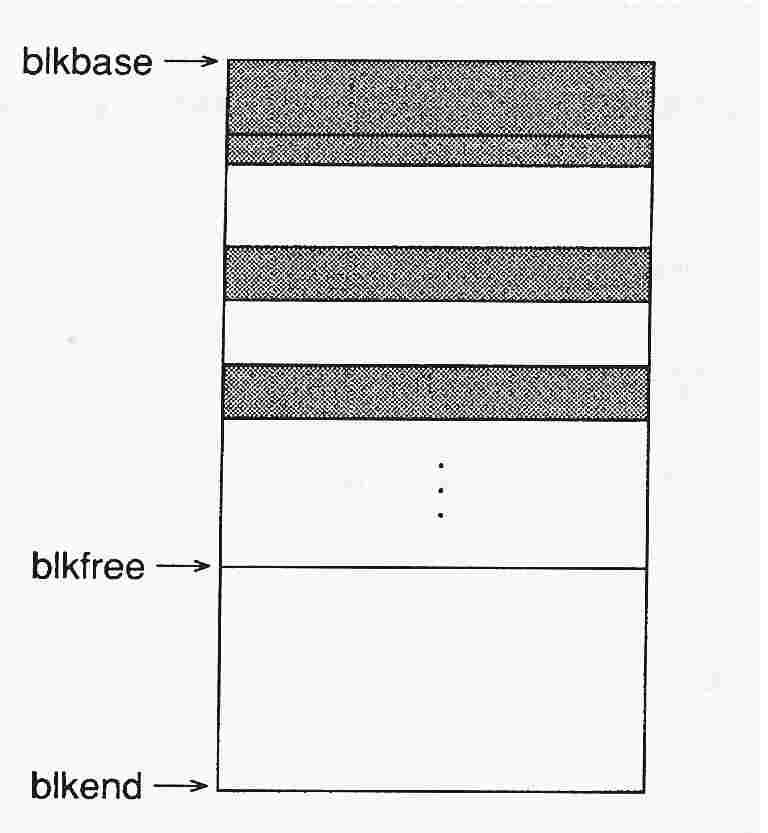
\includegraphics[width=2.5654in,height=2.7811in]{ib-img/ib-img102.jpg} 
\definecolor{lightgrey}{RGB}{180,180,180}
\begin{picture}(300,200)
\thicklines
\put(80,183){\vector(1,0){20}}
\put(75,183){\makebox(0,0)[r]{\texttt{blkbase}}}
\put(80,50){\vector(1,0){20}}
\put(75,50){\makebox(0,0)[r]{\texttt{blkfree}}}
\put(150,65){\vdots}
\put(80,0){\vector(1,0){20}}
\put(75,0){\makebox(0,0)[r]{\texttt{blkend}}}
\put(100,50){\line(1,0){106}}
\put(100,0){\frame{\makebox(106,183){}}}
\put(100,160){\colorbox{lightgrey}{\makebox(100,20){}}}
\put(100,120){\colorbox{lightgrey}{\makebox(100,16){}}}
\put(100,117){\line(1,0){106}}
\put(100,139){\line(1,0){106}}
\put(100,90){\colorbox{lightgrey}{\makebox(100,8){}}}
\put(100,87){\line(1,0){106}}
\put(100,101){\line(1,0){106}}
\linethickness{1.2pt}
\put(100,165){\line(1,0){106}}
\end{picture}

In the allocated block region, pointer adjustment and compaction are
done in two linear passes over the region between \texttt{blkbase} and
\texttt{blkfree}. In the first pass, two pointers are used,
\texttt{dest} and \texttt{source}.  \texttt{dest} points to where the
next block will be after blocks are moved in the next pass, while
\texttt{source} points to the next block to be processed. Both
\texttt{dest} and source start at \texttt{blkbase}, pointing to the
first allocated block.

During this pass, the title of each block pointed to by
\texttt{source} is examined. If it is not marked (that is, if it is
not larger than the maximum type code), \texttt{dest} is left
unchanged and \texttt{source} is incremented by the size of the block
to get to the title of the next block. Thus, unmarked blocks are
skipped. The array \texttt{bsizes} is used, as before, to determine
block sizes.

If the title of the block pointed to by \texttt{source} is marked, its
back chain of descriptors is processed, changing their v-words to
point to where \texttt{dest} points. 
Version 6 of Icon (where some variable descriptors pointed to {\em
  within} blocks) needed to treat such descriptors specially to
account for the extra offset. A previous edition of this book said
\begin{quote}
``A variable descriptor that points to a descriptor in a structure
points \textit{within} a block, not to the title of a block. This is
the only case in which the offset, which is contained in the
least-significant portion of the d-word of a non-trapped-variable
descriptor, is nonzero. Consequently, this offset is used to
distinguish such variables.''

\hspace*{2.5in} \vdots

``In the case of a variable descriptor that is not a trapped-variable
descriptor, the offset in its d-word is added to its v-word, so that
it points to the appropriate relative position with respect to
\texttt{dest}.''
\end{quote}
Unfortunately in version 8 of Icon, which substituted block-pointers
for the descriptors in blocks that pointed to other blocks (and hence
introduced block-pointers into the back chain), it is no longer
possible to identify offset descriptors because the value of the word
immediately before the pointer in the chain can no longer be
guaranteed to be the d-word of a descriptor. As a consequence, {\em
  all} descriptors now point to the start of the block, so the
previous special case is no longer neccessary. The previous treatment
of offset descriptors was an optimization for speed of access during
normal execution. With the introduction of block-pointers, which make
all blocks smaller, we have effectively traded a reduction in space
for all programs for a slightly increased execution time in some
cases.

The last descriptor in the back chain is identified by the fact that
its v-word contains a type code (a value smaller than any possible
pointer to the allocated block region). This type code is restored to
the title of the block before the v-word is changed to point to the
destination. An m flag is set in the title to distinguish it as a
marked block, since the former marking method no longer applies, but
the compaction phase needs to determine which blocks are to be moved.

After the back chain has been processed, all descriptors that point to
the block now point to where the block \textit{will be }when it is
moved during the compaction phase. The block itself is not moved at
this time. This is illustrated by the example given previously, in
which three descriptors point to a record block. After marking, the
situation is

%--%\ \  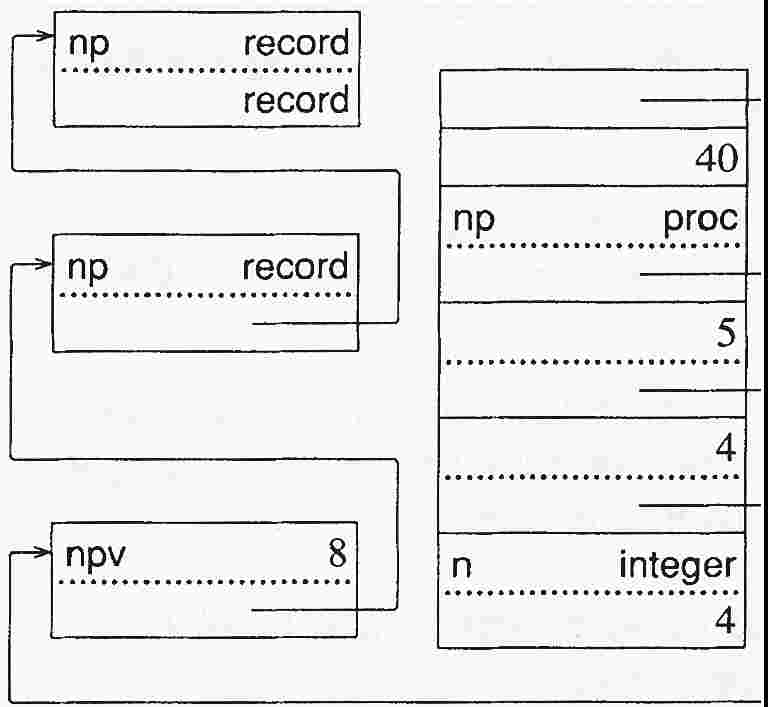
\includegraphics[width=2.5654in,height=2.3602in]{ib-img/ib-img103.jpg} 
\begin{picture}(300,220)(-20,-20)
\put(140,128){\blkbox{}{40}}
\put(140,112){\wordbox{\textit{id}}}
\put(140,96){\wordbox{proc}}
\put(320,96){\wordbox{}}
\put(320,96){\downetc}
\put(320,110){\makebox(100,16){record-constructor}}
\put(346,104){\vector(-1,0){106}}
\put(140,64){\dvboxptr{5}{}{40}{\texttt{"chair"}}}
\put(140,32){\dvboxptr{4}{}{40}{\texttt{"noun"}}}
\put(140,0){\dvbox{integer}{n}{4}}
\put(0,80){\dvbox{record}{np}{}}
\put(0,80){\tlboxlabel{\texttt{y}{\hspace{20pt}}}}
\put(0,144){\tlboxlabel{\texttt{x}{\hspace{20pt}}}}
\put(0,144){\dvbox{record}{np}{record}{}}
\put(0,16){\dvbox{8}{npv}{}}
\put(80,88){\line(1,0){40}}
\put(120,88){\line(0,1){40}}
\put(120,128){\line(-1,0){140}}
\put(-20,128){\line(0,1){42}}
\put(220,154){\line(1,0){95}}
\put(315,154){\line(0,-1){48}}
\put(315,104){\oval(4,4)[r]}
\put(315,102){\line(0,-1){118}}
\put(315,-16){\line(-1,0){335}}
\put(-20,-16){\line(0,1){56}}
\put(-20,170){\vector(1,0){20}}
\put(-20,40){\vector(1,0){20}}
\put(80,24){\line(1,0){40}}
\put(120,24){\line(0,1){40}}
\put(120,64){\line(-1,0){140}}
\put(-20,64){\line(0,1){40}}
\put(-20,104){\vector(1,0){20}}
\end{picture}

\noindent After processing the back chain, the situation is

%--%\ \  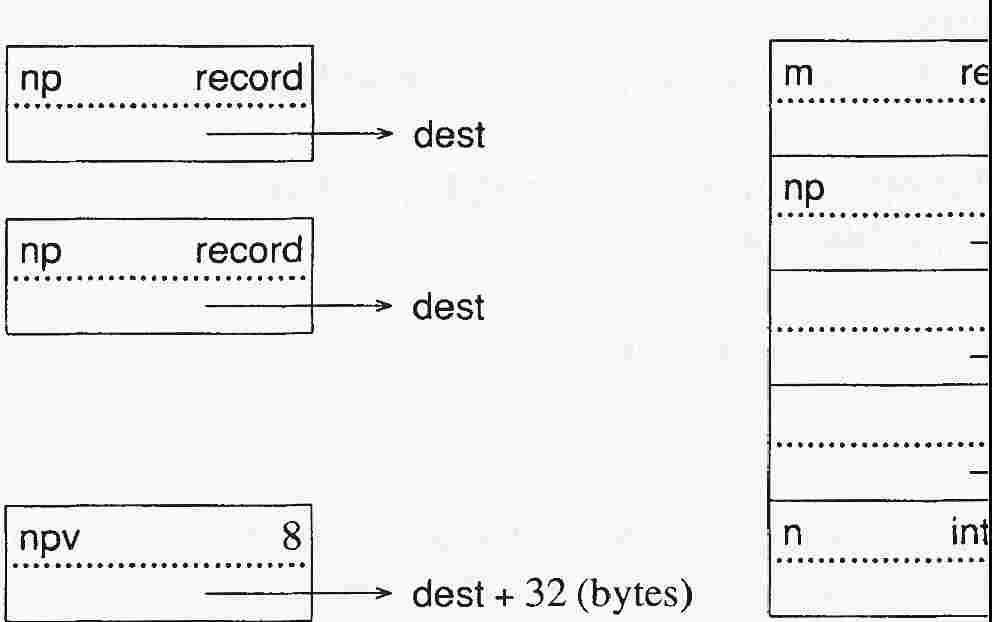
\includegraphics[width=3.3134in,height=2.0772in]{ib-img/ib-img104.jpg} 
\begin{picture}(300,220)(20,0)
\begin{picture}(0,0)(-30,-10)
\put(140,128){\dvbox{record}{m}{40}}
\put(140,112){\wordbox{\textit{id}}}
\put(140,96){\wordbox{proc}}
\put(320,96){\wordbox{}}
\put(320,96){\downetc}
\put(320,110){\makebox(100,16){record-constructor}}
\put(346,104){\vector(-1,0){106}}
\put(140,64){\dvboxptr{5}{}{40}{\texttt{"chair"}}}
\put(140,32){\dvboxptr{4}{}{40}{\texttt{"noun"}}}
\put(140,0){\dvbox{integer}{n}{4}}
\end{picture}
\put(0,80){\dvboxptr{record}{np}{40}{\texttt{dest}}}
\put(0,144){\dvboxptr{record}{np}{40}{\texttt{dest}}}
\put(0,16){\dvboxptr{8}{npv}{40}{\texttt{dest}}}
\end{picture}

\noindent Note that the v-words of the descriptors point to where the
block \textit{will be} after it is moved. When the record constructor
block is encountered and processed (assuming the value of
\texttt{dest} at that time is \texttt{dest\_rc}), the situation
becomes

\begin{picture}(300,210)(20,0)
\begin{picture}(0,0)(-36,-10)
\put(140,128){\dvbox{record}{m}{40}}
\put(140,112){\wordbox{\textit{id}}}
\put(140,96){\wordboxptr{50}{\texttt{dest\_rc}}}
\put(140,64){\dvboxptr{5}{}{40}{\texttt{"chair"}}}
\put(140,32){\dvboxptr{4}{}{40}{\texttt{"noun"}}}
\put(140,0){\dvbox{integer}{n}{4}}
\end{picture}
\begin{picture}(0,0)(0,-56)
\put(320,96){\wordbox{proc}}
\put(320,96){\downetc}
\put(320,110){\makebox(100,16){record-constructor}}
\end{picture}
\begin{picture}(0,0)
\put(0,80){\dvboxptr{record}{np}{40}{\texttt{dest}}}
\put(0,144){\dvboxptr{record}{np}{40}{\texttt{dest}}}
\put(0,16){\dvboxptr{8}{npv}{40}{\texttt{dest}}}
\end{picture}
\end{picture}


The routine for adjusting pointers to the allocated block region is

%-% {\ttfamily\mdseries
%-% static void adjust(char *source, char *dest)
%-% }
%-% 
%-% {\ttfamily\mdseries
%-% \ \ \ \{
%-% }
%-% 
%-% {\ttfamily\mdseries
%-% \ \ \ register union block **nxtptr, **tptr;
%-% }
%-% 
%-% \bigskip
%-% 
%-% {\ttfamily\mdseries
%-% \ \ \ /*
%-% }
%-% 
%-% {\ttfamily\mdseries
%-% \ \ \ \ * Loop through to the end of allocated block region, moving}
%-% 
%-% {\ttfamily\mdseries
%-% \ \ \ \ * \ source to each block in turn and using the size of a block}
%-% 
%-% {\ttfamily\mdseries
%-% \ \ \ \ * \ to find the next block.
%-% }
%-% 
%-% {\ttfamily\mdseries
%-% \ \ \ \ */
%-% }
%-% 
%-% {\ttfamily\mdseries
%-% \ \ \ while (source {\textless} blkfree) \{
%-% }
%-% 
%-% {\ttfamily\mdseries
%-% \ \ \ \ \ \ if ((uword)(nxtptr = (union block **)BlkType(source)) {\textgreater}}
%-% 
%-% {\ttfamily\mdseries
%-% \ \ \ \ \ \ \ \ \ \ \ MaxType) \{}
%-% 
%-% 
%-% \bigskip
%-% 
%-% {\ttfamily\mdseries
%-% \ \ \ \ \ \ \ \ \ /*
%-% }
%-% 
%-% {\ttfamily\mdseries
%-% \ \ \ \ \ \ \ \ \ \ * The type field of source is a back pointer. Traverse}
%-% 
%-% {\ttfamily\mdseries
%-% \ \ \ \ \ \ \ \ \ \ * \ the chain of back pointers, changing each block}
%-% 
%-% {\ttfamily\mdseries
%-% \ \ \ \ \ \ \ \ \ \ * \ location from source to dest.
%-% }
%-% 
%-% {\ttfamily\mdseries
%-% \ \ \ \ \ \ \ \ \ \ */
%-% }
%-% 
%-% {\ttfamily\mdseries
%-% \ \ \ \ \ \ \ \ \ while ((uword)nxtptr {\textgreater} MaxType) \{
%-% }
%-% 
%-% {\ttfamily\mdseries
%-% \ \ \ \ \ \ \ \ \ \ \ \ tptr = nxtptr;
%-% }
%-% 
%-% {\ttfamily\mdseries
%-% \ \ \ \ \ \ \ \ \ \ \ \ nxtptr = (union block **) *nxtptr;
%-% }
%-% 
%-% {\ttfamily\mdseries
%-% \ \ \ \ \ \ \ \ \ \ \ \ *tptr = (union block *)dest;
%-% }
%-% 
%-% {\ttfamily\mdseries
%-% \ \ \ \ \ \ \ \ \ \ \ \ \}
%-% }
%-% 
%-% {\ttfamily\mdseries
%-% \ \ \ \ \ \ \ \ \ BlkType(source) = (uword)nxtptr {\textbar} F\_Mark;
%-% }
%-% 
%-% {\ttfamily\mdseries
%-% \ \ \ \ \ \ \ \ \ dest += BlkSize(source);
%-% }
%-% 
%-% {\ttfamily\mdseries
%-% \ \ \ \ \ \ \ \ \ \}
%-% }
%-% 
%-% {\ttfamily\mdseries
%-% \ \ \ \ \ \ source += BlkSize(source);
%-% }
%-% 
%-% {\ttfamily\mdseries
%-% \ \ \ \ \ \ \}
%-% }
%-% 
%-% {\ttfamily\mdseries
%-% \ \ \ \}}
\goodbreak
\iconcode{
static void adjust(char *source, char *dest)\\
\>\{\\
\>register union block **nxtptr, **tptr;\\
\\
\>/*\\
\>\ * Loop through to the end of allocated block region, moving\\
\>\ * \ source to each block in turn and using the size of a block\\
\>\ * \ to find the next block.\\
\>\ */\\
\>while (source < blkfree) \{\\
\>\>if ((uword)(nxtptr = (union block **)BlkType(source)) >\\
\>\>\>\ \ MaxType) \{\\
\\
\>\>\>/*\\
\>\>\>\ * The type field of source is a back pointer. Traverse\\
\>\>\>\ * \ the chain of back pointers, changing each block\\
\>\>\>\ * \ location from source to dest.\\
\>\>\>\ */\\
\>\>\>while ((uword)nxtptr > MaxType) \{\\
\>\>\>\>tptr = nxtptr;\\
\>\>\>\>nxtptr = (union block **) *nxtptr;\\
\>\>\>\>*tptr = (union block *)dest;\\
\>\>\>\>\}\\
\>\>\>BlkType(source) = (uword)nxtptr | F\_Mark;\\
\>\>\>dest += BlkSize(source);\\
\>\>\>\}\\
\>\>source += BlkSize(source);\\
\>\>\}\\
\>\}
}

When the pointer-adjustment phase is complete, the blocks can be
moved. At this time, all the block titles contain type codes, and
those that are to be saved are marked by m flags. During the
compaction phase, these pointers are used again to reference the
destination and source of blocks to be moved.

If an unmarked block is encountered, source is incremented by the
block skipping over the block. If a marked block is encountered, the m
flag in its is removed and the block is copied to \texttt{dest}. Then
\texttt{dest} and \texttt{source} are incremented by the size of the
block.

When \texttt{blkfree} is reached, it is set to \texttt{dest}. At this
point the allocated block region has been compacted. All saved blocks
are before \texttt{blkfree}, and all free space is after it. The
pointers that were adjusted now point to their blocks, and the
relative situation is the same as it was before garbage collection.

The routine for compacting the allocated block region is

%-% {\ttfamily\mdseries
%-% static void compact(source)
%-% }
%-% 
%-% {\ttfamily\mdseries
%-% char *source;
%-% }
%-% 
%-% {\ttfamily\mdseries
%-% \ \ \ \{
%-% }
%-% 
%-% {\ttfamily\mdseries
%-% \ \ \ register char *dest;
%-% }
%-% 
%-% {\ttfamily\mdseries
%-% \ \ \ register word size;
%-% }
%-% 
%-% \bigskip
%-% 
%-% {\ttfamily\mdseries
%-% \ \ \ /*
%-% }
%-% 
%-% {\ttfamily\mdseries
%-% \ \ \ \ * Start dest at source.
%-% }
%-% 
%-% {\ttfamily\mdseries
%-% \ \ \ \ */
%-% }
%-% 
%-% {\ttfamily\mdseries
%-% \ \ \ dest = source;
%-% }
%-% 
%-% 
%-% \bigskip
%-% 
%-% {\ttfamily\mdseries
%-% \ \ \ /*
%-% }
%-% 
%-% {\ttfamily\mdseries
%-% \ \ \ \ * Loop through to end of allocated block space, moving source}
%-% 
%-% {\ttfamily\mdseries
%-% \ \ \ \ * \ to each block in turn, using the size of a block to find}
%-% 
%-% {\ttfamily\mdseries
%-% \ \ \ \ * \ the next block. If a block has been marked, it is copied}
%-% 
%-% {\ttfamily\mdseries
%-% \ \ \ \ * \ to the location pointed to by dest and dest is pointed}
%-% 
%-% {\ttfamily\mdseries
%-% \ \ \ \ * \ past the end of the block, which is the location to place}
%-% 
%-% {\ttfamily\mdseries
%-% \ \ \ \ * \ the next saved block. \ Marks are removed from the saved}
%-% 
%-% {\ttfamily\mdseries
%-% \ \ \ \ * \ blocks.}
%-% 
%-% {\ttfamily\mdseries
%-% \ \ \ \ */
%-% }
%-% 
%-% {\ttfamily\mdseries
%-% \ \ \ while (source {\textless} blkfree) \{
%-% }
%-% 
%-% {\ttfamily\mdseries
%-% \ \ \ \ \ \ size = BlkSize(source);
%-% }
%-% 
%-% {\ttfamily\mdseries
%-% \ \ \ \ \ \ if (BlkType(source) \& F\_Mark) \{
%-% }
%-% 
%-% {\ttfamily\mdseries
%-% \ \ \ \ \ \ \ \ \ BlkType(source) \&= \~{}F\_Mark;
%-% }
%-% 
%-% {\ttfamily\mdseries
%-% \ \ \ \ \ \ \ \ \ if (source != dest)
%-% }
%-% 
%-% {\ttfamily\mdseries
%-% \ \ \ \ \ \ \ \ \ \ \ \ mvc((uword)size,source,dest);
%-% }
%-% 
%-% {\ttfamily\mdseries
%-% \ \ \ \ \ \ \ \ \ dest += size;
%-% }
%-% 
%-% {\ttfamily\mdseries
%-% \ \ \ \ \ \ \ \ \ \}
%-% }
%-% 
%-% {\ttfamily\mdseries
%-% \ \ \ \ \ \ source += size;
%-% }
%-% 
%-% {\ttfamily\mdseries
%-% \ \ \ \ \ \ \}
%-% }
%-% 
%-% 
%-% \bigskip
%-% 
%-% {\ttfamily\mdseries
%-% \ \ \ /*
%-% }
%-% 
%-% {\ttfamily\mdseries
%-% \ \ \ \ * dest is the location of the next free block. Now that}
%-% 
%-% {\ttfamily\mdseries
%-% \ \ \ \ * \ compaction is complete, point blkfree to that location.
%-% }
%-% 
%-% {\ttfamily\mdseries
%-% \ \ \ \ */
%-% }
%-% 
%-% {\ttfamily\mdseries
%-% \ \ \ blkfree = dest;
%-% }
%-% 
%-% {\ttfamily\mdseries
%-% \ \ \ \}}
\goodbreak
\iconcode{
static void compact(source)\\
char *source;\\
\{\\
\>register char *dest;\\
\>register word size;\\
\\
\>/*\\
\>\ * Start dest at source.\\
\>\ */\\
\>dest = source;\\
\\
\>/*\\
\>\ * Loop through to end of allocated block space, moving source\\
\>\ * \ to each block in turn, using the size of a block to find\\
\>\ * \ the next block. If a block has been marked, it is copied\\
\>\ * \ to the location pointed to by dest and dest is pointed\\
\>\ * \ past the end of the block, which is the location to place\\
\>\ * \ the next saved block. \ Marks are removed from the saved\\
\>\ * \ blocks.\\
\>\ */\\
\>while (source < blkfree) \{\\
\>\>size = BlkSize(source);\\
\>\>if (BlkType(source) \& F\_Mark) \{\\
\>\>\>BlkType(source) \&= \~{}F\_Mark;\\
\>\>\>if (source != dest)\\
\>\>\>\>mvc((uword)size,source,dest);\\
\>\>\>dest += size;\\
\>\>\>\}\\
\>\>source += size;\\
\>\>\}\\
\\
\>/*\\
\>\ * dest is the location of the next free block. Now that\\
\>\ * \ compaction is complete, point blkfree to that location.\\
\>\ */\\
\>blkfree = dest;\\
\}
}

The routine \texttt{mvc(n, source, dest)} moves n bytes from source to dest.

\subsection[11.3.4 Collecting Co-Expression Blocks]{11.3.4 Collecting Co-Expression Blocks}

After the location phase of garbage collection is complete, all the
live co-expression blocks are marked, but the dead co-expression
blocks are not. It is a simple matter to process the list of
co-expression blocks, which are linked by pointers, calling \texttt{free} to
deallocate dead ones and at the same time removing them from the
list. For live co-expressions, the type code in the title is
restored. The routine \texttt{cofree} that frees co-expression blocks is

%-% {\ttfamily\mdseries
%-% \ \ \ static void cofree()}
%-% 
%-% {\ttfamily\mdseries
%-% \ \ \ \{}
%-% 
%-% {\ttfamily\mdseries
%-% \ \ \ register struct b\_coexpr **ep, *xep;}
%-% 
%-% 
%-% \bigskip
%-% 
%-% {\ttfamily\mdseries
%-% \ \ \ /*}
%-% 
%-% {\ttfamily\mdseries
%-% \ \ \ \ * Reset the type for \&main.}
%-% 
%-% {\ttfamily\mdseries
%-% \ \ \ \ */}
%-% 
%-% {\ttfamily\mdseries
%-% \ \ \ BlkLoc(k\_main)-{\textgreater}coexpr.titie = T\_Coexpr;}
%-% 
%-% {\ttfamily\mdseries
%-% \ \ \ /*}
%-% 
%-% {\ttfamily\mdseries
%-% \ \ \ \ * The co-expression blocks are linked together through their}
%-% 
%-% {\ttfamily\mdseries
%-% \ \ \ \ * nextstk fields, with stklist pointing to the head of the}
%-% 
%-% {\ttfamily\mdseries
%-% \ \ \ \ * list. The list is traversed and each stack that was not}
%-% 
%-% {\ttfamily\mdseries
%-% \ \ \ \ * marked is freed.}
%-% 
%-% {\ttfamily\mdseries
%-% \ \ \ \ */}
%-% 
%-% {\ttfamily\mdseries
%-% \ \ \ ep = \&stklist;}
%-% 
%-% {\ttfamily\mdseries
%-% \ \ \ while (*ep != NULL) \{}
%-% 
%-% {\ttfamily\mdseries
%-% \ \ \ \ \ \ if (BlkType(*ep) == T\_Coexpr) \{}
%-% 
%-% {\ttfamily\mdseries
%-% \ \ \ \ \ \ \ \ \ xep = *ep;}
%-% 
%-% {\ttfamily\mdseries
%-% \ \ \ \ \ \ \ \ \ *ep = (*ep)-{\textgreater}nextstk;}
%-% 
%-% {\ttfamily\mdseries
%-% \ \ \ \ \ \ \ \ \ /*
%-% }
%-% 
%-% {\ttfamily\mdseries
%-% \ \ \ \ \ \ \ \ \ \ * Free the astkblks. There should always be one and it}
%-% 
%-% {\ttfamily\mdseries
%-% \ \ \ \ \ \ \ \ \ \ * \ seems that it's not possible to have more than one,}
%-% 
%-% {\ttfamily\mdseries
%-% \ \ \ \ \ \ \ \ \ \ * \ but nonetheless, the code provides for more than one}
%-% 
%-% {\ttfamily\mdseries
%-% \ \ \ \ \ \ \ \ \ \ */
%-% }
%-% 
%-% {\ttfamily\mdseries
%-% \ \ \ \ \ \ \ \ \ for (abp = xep-{\textgreater}es\_actstk; abp; ) \{
%-% }
%-% 
%-% {\ttfamily\mdseries
%-% \ \ \ \ \ \ \ \ \ \ \ \ xabp = abp;
%-% }
%-% 
%-% {\ttfamily\mdseries
%-% \ \ \ \ \ \ \ \ \ \ \ \ abp = abp-{\textgreater}astk\_nxt;
%-% }
%-% 
%-% {\ttfamily\mdseries
%-% \ \ \ \ \ \ \ \ \ \ \ \ free((pointer)xabp);
%-% }
%-% 
%-% {\ttfamily\mdseries
%-% \ \ \ \ \ \ \ \ \ \ \ \ \}
%-% }
%-% 
%-% {\ttfamily\mdseries
%-% \ \ \ \ \ \ \ \ \ coclean(xep-{\textgreater}cstate); }
%-% 
%-% {\ttfamily\mdseries
%-% \ \ \ \ \ \ \ \ \ free((char *)xep);}
%-% 
%-% {\ttfamily\mdseries
%-% \ \ \ \ \ \ \ \ \ \}}
%-% 
%-% {\ttfamily\mdseries
%-% \ \ \ \ \ \ else \{}
%-% 
%-% {\ttfamily\mdseries
%-% \ \ \ \ \ \ \ \ \ BlkType(*ep) = T\_Coexpr;}
%-% 
%-% {\ttfamily\mdseries
%-% \ \ \ \ \ \ \ \ \ ep = \&(*ep)-{\textgreater}nextstk;}
%-% 
%-% {\ttfamily\mdseries
%-% \ \ \ \ \ \ \ \ \ \}}
%-% 
%-% {\ttfamily\mdseries
%-% \ \ \ \ \ \ \}}
%-% 
%-% {\ttfamily\mdseries
%-% \ \ \ \}}
\bigskip
\goodbreak
\iconcode{
static void cofree()\\
\{\\
\>register struct b\_coexpr **ep, *xep;\\
\\
\>/*\\
\>\ * Reset the type for \&main.\\
\>\ */\\
\>BlkLoc(k\_main)->coexpr.titie = T\_Coexpr;\\
\>/*\\
\>\ * The co-expression blocks are linked together through their\\
\>\ * nextstk fields, with stklist pointing to the head of the\\
\>\ * list. The list is traversed and each stack that was not\\
\>\ * marked is freed.\\
\>\ */\\
\>ep = \&stklist;\\
\>while (*ep != NULL) \{\\
\>\>if (BlkType(*ep) == T\_Coexpr) \{\\
\>\>\>xep = *ep;\\
\>\>\>*ep = (*ep)->nextstk;\\
\>\>\>/*\\
\>\>\>\ * Free the astkblks. There should always be one and it\\
\>\>\>\ * \ seems that it's not possible to have more than one,\\
\>\>\>\ * \ but nonetheless, the code provides for more than one\\
\>\>\>\ */\\
\>\>\>for (abp = xep->es\_actstk; abp; ) \{\\
\>\>\>\>xabp = abp;\\
\>\>\>\>abp = abp->astk\_nxt;\\
\>\>\>\>free((pointer)xabp);\\
\>\>\>\>\}\\
\>\>\>coclean(xep->cstate); \\
\>\>\>free((char *)xep);\\
\>\>\>\}\\
\>\>else \{\\
\>\>\>BlkType(*ep) = T\_Coexpr;\\
\>\>\>ep = \&(*ep)->nextstk;\\
\>\>\>\}\\
\>\>\}\\
\}
}

\subsection[11.3.5 Multiple Regions]{11.3.5 Multiple Regions}

Garbage collection may not produce enough free space in a region to
satisfy the request that caused the garbage collection. In this case,
the region for which the request was made is replaced with a new
larger region. In addition, the allocated string and block regions are
replaced if the amount of free space in them after garbage collection
otherwise would be less than a minimum value, which is called
``breathing room.'' This attempts to avoid ``thrashing'' that might
result from a garbage collection that leaves a small amount of free
space, only to result in a subsequent garbage collection almost
immediately.

The set of string and block regions for a program are managed as a
linked list. Older, ``tenured'' regions are revisited, and garbage
collected, prior to allocating new, larger regions. If an older region
frees enough space, it is made the active region instead of allocating
a new one.

\subsection[11.3.6 Storage Requirements during Garbage Collection]{11.3.6 Storage Requirements during Garbage Collection}

Garbage collection itself takes some work space. Space for pointers to
qualifiers is provided in \texttt{quallist}, while C stack space is
needed for calls to routine that perform the various aspects of
garbage collection, which are heavily recursive.

The space for \texttt{quallist} is obtained from the free space at the
end of the allocated block region. The amount of space needed is
proportional to the number of qualifiers whose v-words point to
strings in the allocated string region and usually is comparatively
small. Space for \texttt{quallist} is obtained in small increments

This is done in \texttt{postqual()}, for which the complete routine is

%-% {\ttfamily\mdseries
%-% static void postqual(dptr dp)}
%-% 
%-% {\ttfamily\mdseries
%-% \ \ \ \{}
%-% 
%-% {\ttfamily\mdseries
%-% \ \ \ char *newqual;}
%-% 
%-% 
%-% \bigskip
%-% 
%-% {\ttfamily\mdseries
%-% \ \ \ if (InRange(strbase,StrLoc(*dp),strfree + 1)) \{}
%-% 
%-% {\ttfamily\mdseries
%-% \ \ \ \ \ \ /*}
%-% 
%-% {\ttfamily\mdseries
%-% \ \ \ \ \ \ \ * The string is in the string space. \ Add it to the string \ \ \ \ }
%-% 
%-% {\ttfamily\mdseries
%-% \ \ \ \ \ \ \ * \ qualifier list, but before adding it, expand the string \ \ \ \ \ \ }
%-% 
%-% {\ttfamily\mdseries
%-% \ \ \ \ \ \ \ * \ qualifier list if necessary.
%-% }
%-% 
%-% {\ttfamily\mdseries
%-% \ \ \ \ \ \ \ */
%-% }
%-% 
%-% {\ttfamily\mdseries
%-% \ \ \ \ \ \ if (qualfree {\textgreater}= equallist) \{
%-% }
%-% 
%-% 
%-% \bigskip
%-% 
%-% {\ttfamily\mdseries
%-% \ \ \ \ \ \ \ \ \ /* reallocate a qualifier list that's twice as large */}
%-% 
%-% {\ttfamily\mdseries
%-% \ \ \ \ \ \ \ \ \ newqual = realloc(quallist, 2 * qualsize);}
%-% 
%-% {\ttfamily\mdseries
%-% \ \ \ \ \ \ \ \ \ if (newqual) \{
%-% }
%-% 
%-% {\ttfamily\mdseries
%-% \ \ \ \ \ \ \ \ \ \ \ \ quallist = (dptr *)newqual;
%-% }
%-% 
%-% {\ttfamily\mdseries
%-% \ \ \ \ \ \ \ \ \ \ \ \ qualfree = (dptr *)(newqual + qualsize);}
%-% 
%-% {\ttfamily\mdseries
%-% \ \ \ \ \ \ \ \ \ \ \ \ qualsize *= 2;
%-% }
%-% 
%-% {\ttfamily\mdseries
%-% \ \ \ \ \ \ \ \ \ \ \ \ equallist = (dptr *)(newqual + qualsize);}
%-% 
%-% {\ttfamily\mdseries
%-% \ \ \ \ \ \ \ \ \ \ \ \ \}
%-% }
%-% 
%-% {\ttfamily\mdseries
%-% \ \ \ \ \ \ \ \ \ else \{
%-% }
%-% 
%-% {\ttfamily\mdseries
%-% \ \ \ \ \ \ \ \ \ \ \ \ qualfail = 1;
%-% }
%-% 
%-% {\ttfamily\mdseries
%-% \ \ \ \ \ \ \ \ \ \ \ \ return;
%-% }
%-% 
%-% {\ttfamily\mdseries
%-% \ \ \ \ \ \ \ \ \ \ \ \ \}
%-% }
%-% 
%-% {\ttfamily\mdseries
%-% \ \ \ \ \ \ \ \ \ \}}
%-% 
%-% {\ttfamily\mdseries
%-% \ \ \ \ \ \ *qualfree++ = dp;}
%-% 
%-% {\ttfamily\mdseries
%-% \ \ \ \ \ \ \}}
%-% 
%-% {\ttfamily\mdseries
%-% \ \ \ \}}
\goodbreak
\iconcode{
static void postqual(dptr dp)\\
\>\{\\
\>char *newqual;\\
\\
\>if (InRange(strbase,StrLoc(*dp),strfree + 1)) \{\\
\>\>/*\\
\>\>\ * The string is in the string space. \ Add it to the string\\
\>\>\ * \ qualifier list, but before adding it, expand the string\\
\>\>\ * \ qualifier list if necessary.\\
\>\>\ */\\
\>\>if (qualfree >= equallist) \{\\
\>\>\>/* reallocate a qualifier list that's twice as large */\\
\>\>\>newqual = realloc(quallist, 2 * qualsize);\\
\>\>\>if (newqual) \{\\
\>\>\>\>quallist = (dptr *)newqual;\\
\>\>\>\>qualfree = (dptr *)(newqual + qualsize);\\
\>\>\>\>qualsize *= 2;\\
\>\>\>\>equallist = (dptr *)(newqual + qualsize);\\
\>\>\>\>\}\\
\>\>\>else \{\\
\>\>\>\>qualfail = 1;\\
\>\>\>\>return;\\
\>\>\>\>\}\\
\>\>\>\}\\
\>\>*qualfree++ = dp;\\
\>\>\}\\
\>\}
}

The amount of stack space required during garbage collection depends
primarily on the depth of recursion in calls to \texttt{markblock()}
and \texttt{markptr()}. Recursion in these functions corresponds to
linked lists of pointers in allocated storage. It occurs where a
descriptor in the static region or the allocated block region points
to an as-yet unmarked block. C stack overflow may occur during garbage
collection. This problem is particularly serious on computers with
small address spaces for programs that use a large amount of allocated
data. The use of stack space during marking is minimized by testing
descriptor v-words before calling \texttt{markblock()}, by using
static storage for variables in \texttt{markblock()} that are not
needed in recursive calls, and by incorporating the code for
processing co-expression blocks in \texttt{markblock()}, rather than
calling a separate routine.

\section[11.4 Predictive Need]{11.4 Predictive Need}

In most systems that manage allocated storage dynamically, garbage
collections are triggered by allocation requests that cannot be
satisfied by the amount of free storage that remains. In these
systems, garbage collections occur during calls to allocation routines.

Whenever a garbage collection occurs, all potentially accessible data
must be reachable from the basis, and any descriptors that are
reachable from the basis must contain valid data. These requirements
pose serious difficulties, since, in the normal course of computation,
pointers to accessible objects may only exist in registers or on the C
stack as C local variables that the garbage collector has no way of
locating. Furthermore, descriptors that are being constructed may
temporarily hold invalid data. While it is helpful to know that
garbage collection can occur only during calls to allocation routines,
allocation often is done in the midst of other computations. Assuring
that all accessible data is reachable and that all reachable data is
valid can be difficult and prone to error.

For these reasons, Icon uses a slightly different strategy, called
``predictive need,'' for triggering garbage collections. Instead of
garbage collection occurring as a byproduct of an allocation request,
the amount of space needed is requested in advance. There is a
routine, \texttt{reserve(Region,n)}, for reserving space in
advance. This routine checks the specified region to assure the amount
of free space needed is actually available. If it is not, it calls the
garbage collector. The code for \texttt{reserve()} is conceptually

%-% {\ttfamily\mdseries
%-% \ \ \ char *reserve(int r, uword n)}
%-% 
%-% {\ttfamily\mdseries
%-% \ \ \ \{}
%-% 
%-% {\ttfamily\mdseries
%-% \ \ \ if (DiffPtrs(regions[r]-{\textgreater}end,regions[r]-{\textgreater}free {\textless} n)}
%-% 
%-% {\ttfamily\mdseries
%-% \ \ \ \ \ \ collect(r,n);}
%-% 
%-% {\ttfamily\mdseries
%-% \ \ \ return regions[r]-{\textgreater}free;}
%-% 
%-% {\ttfamily\mdseries
%-% \ \ \ \}}
\goodbreak
\iconcode{
\>char *reserve(int r, uword n)\\
\>\{\\
\>\>if (DiffPtrs(regions[r]->end,regions[r]->free < n)\\
\>\>\>collect(r,n);\\
\>\>return regions[r]->free;\\
\>\}
}

\noindent
In practice, things are more complicated, as the current region may be
changed or a new region may be allocated in order to satisfy the
request.


The string allocator mainly ensures space is available and then
updates the free pointer:

%-% {\ttfamily\mdseries
%-% \ \ \ char *alcstr(char *s, word slen)}
%-% 
%-% {\ttfamily\mdseries
%-% \ \ \ \{}
%-% 
%-% {\ttfamily\mdseries
%-% \ \ \ tended struct descrip ts;
%-% }
%-% 
%-% {\ttfamily\mdseries
%-% \ \ \ register char *d;
%-% }
%-% 
%-% {\ttfamily\mdseries
%-% \ \ \ char *ofree;
%-% }
%-% 
%-% 
%-% \bigskip
%-% 
%-% {\ttfamily\mdseries
%-% \ \ \ /*
%-% }
%-% 
%-% {\ttfamily\mdseries
%-% \ \ \ \ * Make sure there is enough room in the string space.}
%-% 
%-% {\ttfamily\mdseries
%-% \ \ \ \ */
%-% }
%-% 
%-% {\ttfamily\mdseries
%-% \ \ \ if (DiffPtrs(strend,strfree) {\textless} slen) \{
%-% }
%-% 
%-% {\ttfamily\mdseries
%-% \ \ \ \ \ \ StrLen(ts) = slen;
%-% }
%-% 
%-% {\ttfamily\mdseries
%-% \ \ \ \ \ \ StrLoc(ts) = s;
%-% }
%-% 
%-% {\ttfamily\mdseries
%-% \ \ \ \ \ \ if (!reserve(Strings, slen))
%-% }
%-% 
%-% {\ttfamily\mdseries
%-% \ \ \ \ \ \ \ \ \ return NULL;
%-% }
%-% 
%-% {\ttfamily\mdseries
%-% \ \ \ \ \ \ s = StrLoc(ts);
%-% }
%-% 
%-% {\ttfamily\mdseries
%-% \ \ \ \ \ \ \}
%-% }
%-% 
%-% 
%-% \bigskip
%-% 
%-% {\ttfamily\mdseries
%-% \ \ \ strtotal += slen;}
%-% 
%-% {\ttfamily\mdseries
%-% \ \ \ /*}
%-% 
%-% {\ttfamily
%-% \ \ \ \ * Copy the string into the string space, saving a pointer to}
%-% 
%-% {\ttfamily\mdseries
%-% \ \ \ \ * its beginning. Note that s may be null, in which case the}
%-% 
%-% {\ttfamily\mdseries
%-% \ \ \ \ * space is still to be allocated but nothing is to be copied}
%-% 
%-% {\ttfamily\mdseries
%-% \ \ \ \ * into it.}
%-% 
%-% {\ttfamily\mdseries
%-% \ \ \ \ */}
%-% 
%-% {\ttfamily\mdseries
%-% \ \ \ ofree = d = strfree;}
%-% 
%-% {\ttfamily\mdseries
%-% \ \ \ if (s) \{}
%-% 
%-% {\ttfamily\mdseries
%-% \ \ \ \ \ \ while (slen-{}- {\textgreater} 0)}
%-% 
%-% {\ttfamily\mdseries
%-% \ \ \ \ \ \ *d++ = *s++;}
%-% 
%-% {\ttfamily\mdseries
%-% \ \ \ \ \ \ \}}
%-% 
%-% {\ttfamily\mdseries
%-% \ \ \ else}
%-% 
%-% {\ttfamily\mdseries
%-% \ \ \ \ \ \ d += slen;}
%-% 
%-% {\ttfamily\mdseries
%-% \ \ \ strfree = d;}
%-% 
%-% {\ttfamily\mdseries
%-% \ \ \ return ofree;}
%-% 
%-% {\ttfamily\mdseries
%-% \ \ \ \}}
\goodbreak
\iconcode{
\>char *alcstr(char *s, word slen)\\
\>\{\\
\>tended struct descrip ts;\\
\>register char *d;\\
\>char *ofree;\\
\\
\>/*\\
\>\ * Make sure there is enough room in the string space.\\
\>\ */\\
\>if (DiffPtrs(strend,strfree) < slen) \{\\
\>\>StrLen(ts) = slen;\\
\>\>StrLoc(ts) = s;\\
\>\>if (!reserve(Strings, slen))\\
\>\>\>return NULL;\\
\>\>s = StrLoc(ts);\\
\>\>\}\\
\\
\>strtotal += slen;\\
\>/*\\
\>\ * Copy the string into the string space, saving a pointer to\\
\>\ * its beginning. Note that s may be null, in which case the\\
\>\ * space is still to be allocated but nothing is to be copied\\
\>\ * into it.\\
\>\ */\\
\>ofree = d = strfree;\\
\>if (s) \{\\
\>\>while (slen-{}- > 0)\\
\>\>*d++ = *s++;\\
\>\>\}\\
\>else\\
\>\>d += slen;\\
\>strfree = d;\\
\>return ofree;\\
\>\}
}

If a garbage collection occurs, a parameter is passed to be sure that
enough space is collected to satisfy any remaining allocation
requests.

Since a predictive need request assures an adequate amount of space,
no garbage collection can occur during the subsequent allocation
request. The advantage of having a garbage collection occur during a
predictive need request rather during an allocation request is that a
safe time can be chosen for a possible garbage collection. The amount
of space needed (or at least an upper bound on it) usually is known
before the storage is actually needed. and when all valid data can be
located from the basis.

A few lines from the implementation of the \texttt{image()} function,
showing how string images are constructed, illustrates predictive
need. The image will consist of a pair of double quotes, enclosing a
representation of the string contents with special characters
escaped. If \texttt{alcstr()} is called separately for the various
components, they might be allocated non-contiguously. Reserving the
maximum space needed ahead of time guarantees subsequent calls to
\texttt{alcstr()} will be contiguous. The maximum needed for image
would be \texttt{StrLen(source)*4+2}, done using a shift operator:

%-% {\ttfamily\mdseries
%-% \ \ \ \ \ \ \ \ \ s = StrLoc(source);
%-% }
%-% 
%-% {\ttfamily\mdseries
%-% \ \ \ \ \ \ \ \ \ len = StrLen(source);
%-% }
%-% 
%-% {\ttfamily\mdseries
%-% \ \ \ \ \ \ \ \ \ Protect (reserve(Strings,(len {\textless}{\textless} 2) + 2), return Error);
%-% }
%-% 
%-% {\ttfamily\mdseries
%-% \ \ \ \ \ \ \ \ \ Protect(t = alcstr({\textquotedbl}{\textbackslash}{\textquotedbl}{\textquotedbl}, (word)(1)), return
%-% Error);}
%-% 
%-% {\ttfamily\mdseries
%-% \ \ \ \ \ \ \ \ \ StrLoc(*dp2) = t;
%-% }
%-% 
%-% {\ttfamily\mdseries
%-% \ \ \ \ \ \ \ \ \ StrLen(*dp2) = 1;
%-% }
%-% 
%-% {\ttfamily\mdseries
%-% \ \ \ \ \ \ \ \ \ while (len-{}- {\textgreater} 0)
%-% }
%-% 
%-% {\ttfamily\mdseries
%-% \ \ \ \ \ \ \ \ \ \ \ \ StrLen(*dp2) += doimage(*s++, '{\textquotedbl}');
%-% }
%-% 
%-% {\ttfamily\mdseries
%-% \ \ \ \ \ \ \ \ \ Protect(alcstr({\textquotedbl}{\textbackslash}{\textquotedbl}{\textquotedbl}, (word)(1)), return
%-% Error);}
%-% 
%-% {\ttfamily\mdseries
%-% \ \ \ \ \ \ \ \ \ ++StrLen(*dp2);}
\goodbreak
\iconcode{
\>\>\>s = StrLoc(source);\\
\>\>\>len = StrLen(source);\\
\>\>\>Protect (reserve(Strings,(len <{}< 2) + 2), return Error);\\
\>\>\>Protect(t = alcstr("{\textbackslash}"", (word)(1)), return Error);\\
\>\>\>StrLoc(*dp2) = t;\\
\>\>\>StrLen(*dp2) = 1;\\
\>\>\>while (len-{}- > 0)\\
\>\>\>\>StrLen(*dp2) += doimage(*s++, '"');\\
\>\>\>Protect(alcstr("{\textbackslash}"", (word)(1)), return Error);\\
\>\>\>++StrLen(*dp2);
}

A disadvantage of predictive need is that the maximum amount of
storage needed must be determined and care must be taken to make
predictive need requests prior to allocation. These problems do not
occur in storage-management systems where garbage collection is
implicit in allocation.


\textsc{Retrospective}: Storage management is one of the major
concerns in the implementation of a run-time system in which space is
allocated dynamically and automatically. Although many programs never
garbage collect at all, for those that do, the cost of garbage
collection may be significant.

The requirements of storage management have a significant influence on
the way that data is represented in Icon, particularly in
blocks. Aspects of data representation that may appear arbitrary in
the absence of considerations related to storage management have
definite uses during garbage collection.

The garbage collector can only identify those pointers of which it is
informed. Globals are informed by placing them in the basis
set. Locals are informed by declaring them to be tended. Descriptors
and block pointers within blocks are specified in tables, indexed by
the block's type code, that describe the number and positional offset
of all pointers within the block.

While it is possible to devise more economical methods of representing
such data at the expense of complexity and loss of generality, any
method of representing data for which space is allocated automatically
has some overhead.

Garbage collection is most expensive when there are many live objects
that must be saved. For programs in which allocated storage is used
transiently and in which there are few live objects, garbage
collection is fast.

\bigskip

\noindent\textbf{EXERCISES}

\noindent {\bf 11.1} Since the first word of a block contains its type
code, why is there also a type code in a descriptor that points to it?

\noindent {\bf 11.2}
{\em Question removed: it no longer applies.}
%% Give an example of an Icon expression that
%% changes the contents of a block that is allocated statically in the
%% run-time system.

\noindent {\bf 11.3} Give an example of an Icon expression that
changes data in the icode region.

\noindent {\bf 11.4} Why not combine global and static identifiers in
a single array of descriptors in the icode region?

\noindent {\bf 11.5} Why are the names of global identifiers needed?

\noindent {\bf 11.6} Why is there no array for the names of static identifiers?

\noindent {\bf 11.7} How long can a string be?

\noindent {\bf 11.8} How many elements can a single list-element block
hold?

\noindent {\bf 11.9} List all the regions of memory in which the
following Icon data objects can occur:
\begin{itemize}
\item 
strings
\item 
descriptors
\item 
co-expression blocks
\item 
other blocks
\end{itemize}

\noindent {\bf 11.10} List all the source-language operations in Icon
that may cause the allocation of storage.

\noindent {\bf 11.11} Give an example of an expression for which it
cannot be determined from the expression itself whether or not it
allocates storage.

\noindent {\bf 11.12} List the block types for which block size may
vary from one block to another.

\noindent {\bf 11.13} List all the types of blocks that may occur in
the allocated block region.

\noindent {\bf 11.14} List all the types of blocks that may occur
outside of the allocated block region.

\noindent {\bf 11.15} Give an example of an Icon program in which the
only access path to a live object during garbage collection is a
variable that points to an element in a structure.

\noindent {\bf 11.16} Give an example of an Icon program that
constructs a circular pointer chain.

\noindent {\bf 11.17} Explain how it can be assured that all blocks in
the allocated block region are at addresses that are larger than the
maximum type code.

\noindent {\bf 11.18} Aside from the possibility of looping in the
location phase of garbage collection, what are the possible
consequences of processing the descriptors in a block more than once?

\noindent {\bf 11.19} What would happen if there were more than one
pointer on quallist to the \textit{same} qualifier?

\noindent {\bf 11.20} Because of the way that the Icon run-time system
is written, blocks that are not in the allocated block region do not
contain pointers to allocated objects. Consequently, the descriptors
in such blocks do not have to be processed during garbage collection.

\begin{itemize}
\item What does this imply about access to such blocks?

\item What changes would have to be made to the garbage collector if
such blocks could contain pointers to allocated objects?

\end{itemize}

\noindent {\bf 11.21}
{\em Question removed: it no longer applies.}
%% There is one exception to the statement in the
%% preceding exercise that blocks that are not in the allocated data
%% region do not contain pointers to allocated objects. Identify this
%% exception and explain how it is handled during garbage collection.

\noindent {\bf 11.22} In the allocated string region, pointer
adjustment and compaction are done in one pass, while two passes are
used in the allocated block region. Why are pointer adjustment and
compaction not done in a single pass over the allocated block region?

\noindent {\bf 11.23} What would be the effect of failing to remove
the m flag from a block title during the compaction of the allocated
block region?

\noindent {\bf 11.24} If garbage collection cannot produce enough free
space in the region for which the collection was triggered, program
execution is terminated even if there is extra space in another
region. Describe how to modify the garbage collector to avoid this
problem.

\noindent {\bf 11.25} Write a program that requires an arbitrarily
large amount of space for quallist.

\noindent {\bf 11.26} Write a program that causes an arbitrary amount
of recursion in markblock during garbage collection.

\noindent {\bf 11.27} Write a program that produces an arbitrarily
large amount of data that must be saved by garbage collection, and
observe the results.

\noindent {\bf 11.28} Devise a more sophisticated method of preventing
thrashing in allocation and garbage collection than the fixed
breathing-room method.

\noindent {\bf 11.29} There is no mechanism to reduce the size of an
allocated region that may be expanded during one garbage collection,
but which has an excessive amount of free space after another garbage
collection. Describe how to implement such a mechanism.

\noindent {\bf 11.30} Suppose that a garbage collection could occur
during a call of any C routine from any other C routine. How would
this complicate the way C routines are written?

\noindent {\bf 11.31} What might happen if

\begin{itemize}

\item The amount of storage specified in a predictive need request
were larger than the amount subsequently allocated?

\item The amount of storage specified in a predictive need request
were smaller than the amount subsequently allocated?

\end{itemize}

\noindent {\bf 11.32} When a list-element block is unlinked as the
result of a pop, get, or pull, can the space it occupies always be
reclaimed by a garbage collection? What are the general considerations
in answering questions such as these?

\noindent {\bf 11.33} A variable that refers to a descriptor in a
block points directly to the descriptor, with an offset in its d-word
to the head of the block in which the descriptor resides. Could it be
the other way around, with a variable pointing to the head of the
block and an offset to the descriptor? If so, what are the advantages
and disadvantages of the two methods?

\noindent {\bf 11.34} Why does sweep process an interpreter stack from
its sp to its base, rather than the other way around?

\noindent {\bf 11.35} As mentioned in Sec. 11.3, all regions are
collected, regardless of the region in which space is needed. Discuss
the pros and cons of this approach.

\noindent {\bf 11.36} Evaluate the cost of using two-word descriptors
for all pointers to blocks, even when these pointers do not correspond
to source-language values (as, for example, in the links among
list-element blocks).

\noindent {\bf 11.37} The need to garbage-collect blocks that are
allocated during program execution significantly affects the structure
and organization of such blocks. Suppose that garbage collection were
never needed. How could the structure and organizations of blocks be
revised to save space?

\noindent {\bf 11.38} Discuss the pros and cons of having different
regions for allocating blocks of different types.

\noindent {\bf 11.39} Some expressions, such as
\iconline{\texttt{while write(read())}}
\noindent result in a substantial amount of ``storage
throughput,'' even though no space really needs to be
allocated. Explain why this effect cannot be avoided in general and
discuss its impact on program performance.

\noindent {\bf 11.40} Physical memory is becoming less and less
expensive, and more computer architectures and operating systems are
providing larger user address spaces. Discuss how very large user
address spaces might affect allocation and garbage-collection
strategies.
